\chapter{Formulazione Teorica e Framework Metodologico}
\label{ch:metodologia}

Il presente capitolo definisce l'impalcatura teorica e il framework metodologico alla base dell'intera indagine sperimentale, fornendo gli strumenti formali necessari per la modellazione, l'analisi e l'adattamento dei sistemi di \textit{Network Intrusion Detection} (NIDS) in contesti operativi eterogenei. 
L'obiettivo primario risiede nella definizione di un paradigma valutativo rigoroso, strutturalmente svincolato dalle specificità implementative dei singoli dataset, che consenta di caratterizzare quantitativamente i fenomeni di traslazione di dominio (\textit{domain shift}) e le prestazioni di generalizzazione, mantenendo distinta la variabilità osservata tra le diverse esecuzioni.

La trattazione si articola secondo una progressione logica suddivisa in quattro sezioni principali:
\begin{itemize}
    \item La \textbf{Sezione~\ref{sec:modello_sistema}} formalizza il modello astratto del sistema, definendo rigorosamente gli spazi vettoriali di rappresentazione, gli operatori di proiezione per l'armonizzazione delle \textit{feature} e le regole architetturali di partizionamento dei domini.
    \item La \textbf{Sezione~\ref{sec:tassonomia_modelli}} delinea la tassonomia delle architetture di classificazione adottate e le relative strategie di \textit{transfer learning}, uniformando le metriche di confronto mediante una formulazione omogenea basata sulla stima della probabilità a posteriori.
    \item La \textbf{Sezione~\ref{sec:framework_adattamento}} stabilisce il protocollo valutativo per la stabilità statistica, affrontando la gestione dell'incertezza stocastica tramite valutazione \textit{multi-seed} e definendo gli indici morfologici di granularità dello spazio decisionale.
    \item Infine, la \textbf{Sezione~\ref{sec:framework_analitico}} completa l'architettura metodologica descrivendo l'apparato diagnostico e di \textit{explainability}, integrando strumenti di stima di densità e metriche di rilevanza fondate sulla teoria dei giochi cooperativi per la caratterizzazione e interpretazione delle divergenze distributive.
\end{itemize}

\section{Modello del Sistema e Spazi di Rappresentazione}
\label{sec:modello_sistema}

La presente sezione formalizza l'impalcatura teorica e matematica del framework analitico, definendo in modo rigoroso gli spazi vettoriali di rappresentazione e le distribuzioni di probabilità necessarie per modellare i fenomeni di transizione cross-dominio nel contesto NIDS delineato nel capitolo precedente.
L'obiettivo è stabilire un modello astratto, indipendente dalle peculiarità di implementazione dei singoli dataset, in grado di garantire il rigore metodologico, la comparabilità delle metriche e l'assenza di contaminazione informativa.

A tal fine, la trattazione introduce preliminarmente la formalizzazione dei domini di origine e destinazione, delineando la semantica a doppia etichettatura $(Y, A)$, le regole di partizionamento preventivo anti-\textit{data leakage} e il vincolo di proporzionamento parametrico $\rho$ alla base delle cinque categorie astratte di benchmark istanziabili dal framework. 
Successivamente, viene definito l'operatore di proiezione $\boldsymbol{\psi}_k$, specifico per ciascun dominio $k \in \{S, T\}$, che mappa le caratteristiche grezze eterogenee nello spazio delle \textit{feature} condiviso $\mathcal{X}$, esplicitando i criteri concettuali di filtraggio e armonizzazione degli attributi. 
La trattazione si conclude motivando, sulla base della proprietà di invarianza rispetto a trasformazioni monotoniche propria dei classificatori a partizionamento ricorsivo, l'omissione della fase esplicita di scalatura dalla definizione dello spazio delle \textit{feature}.

Per facilitare la lettura della trattazione successiva, i principali simboli e costrutti matematici adottati sono sintetizzati nella Tabella~\ref{tab:notazione_matematica}.

\begin{table}[H]
    \centering
    \small
    \caption{Sintesi della notazione matematica e dei simboli del framework.}
    \label{tab:notazione_matematica}
    \begin{tabularx}{\textwidth}{
        >{\raggedright\arraybackslash}p{3cm}
        >{\raggedright\arraybackslash}X
    }
        \toprule
        \textbf{Simbolo} & \textbf{Significato} \\
        \midrule

        $\mathcal{D} = (\mathcal{X}, P(\mathbf{x}))$ &
        Dominio di traffico e relativa distribuzione \\

        $\mathcal{X} \subseteq \mathbb{R}^d$ &
        Spazio condiviso delle \textit{feature} \\

        $\mathbf{x} = (x_1, \dots, x_d)^\top$ &
        Vettore delle \textit{feature} di un flusso \\

        $\mathcal{Y} = \{0,1\}$ &
        Etichetta binaria: $0$ normale, $1$ malevolo \\

        $A \in \mathcal{A}$ &
        Classe specifica del flusso: \textit{Normal} o famiglia d'attacco \\

        $\mathcal{A}_S, \mathcal{A}_T$ &
        Famiglie di attacco sorgente e target \\

        $\mathcal{D}_S, \mathcal{D}_T$ &
        Domini sorgente e target \\

        $\mathcal{D}_k^{(train)}, \mathcal{D}_k^{(test)}$ &
        Partizioni di addestramento e test del dominio $k$ \\

        $\boldsymbol{\psi}_{k \in \{S,T\}}(\cdot)$ &
        Operatore di proiezione nello spazio condiviso $\mathcal{X}$ \\

        $N(\cdot)$ &
        Cardinalità dell'insieme considerato \\

        \bottomrule
    \end{tabularx}
\end{table}

\subsection{Formalizzazione dei Domini e Composizione Asimmetrica del Traffico}
\label{subsec:composizione_domini}

Il framework analitico richiede la definizione rigorosa degli spazi di rappresentazione vettoriale e delle distribuzioni di probabilità associate ai diversi contesti di rete considerati. Si definisce un dominio $\mathcal{D}$ come la coppia $(\mathcal{X}, P(\mathbf{x}))$, dove $\mathcal{X} \subseteq \mathbb{R}^d$ rappresenta lo spazio delle \textit{feature} $d$-dimensionale condiviso e $P(\mathbf{x})$ la distribuzione di probabilità marginale definita sul vettore delle caratteristiche $\mathbf{x} = (x_1, x_2, \dots, x_d)^\top \in \mathcal{X}$.

Associato a ciascun dominio, la semantica del traffico è modellata tramite una doppia etichettatura. Lo spazio discreto primario $\mathcal{Y} = \{0,1\}$ stabilisce la natura del flusso, dove $Y = 0$ indica il traffico nominale (\textit{Normal}) e $Y = 1$ identifica genericamente un vettore malevolo. In aggiunta, si definisce un'ulteriore variabile descrittiva $A \in \mathcal{A}$ che specifica il nome della classe, garantendo una caratterizzazione puntuale sia per la componente benevola ($Y = 0$), per la quale $A$ assume tipicamente un unico valore costante (\textit{Normal}), sia per le diverse famiglie di attacco ($Y = 1$), per le quali $A$ è genuinamente multi-valore.

\subsubsection{Caratterizzazione Astratta dei Domini e Tassonomia delle Classi}
\label{subsubsec:caratterizzazione_domini}
Il framework analitico modella il fenomeno di transizione cross-dominio a partire da due macro-distribuzioni di partenza distinte:
\begin{enumerate}
    \item \textbf{Dominio di Riferimento ($\mathcal{D}_S$):} rappresenta l'ambiente stazionario di origine, contenente sia istanze di traffico nominale ($Y = 0, A = \textit{Normal}$) sia flussi malevoli ($Y = 1, A \in \mathcal{A}_S$). Per eliminare le componenti ad elevata sparsità ed esigua rappresentatività statistica, si applica una procedura di rimozione delle classi minoritarie (\textit{minority removal}) sull'insieme $\mathcal{A}_S$, garantendo una caratterizzazione stabile del baseline di superficie.
    \item \textbf{Domini di Destinazione ($\mathcal{D}_T$):} rappresentano i contesti soggetti a variazioni trasmissive o canali eterogenei, composti esclusivamente da vettori di traffico malevolo ($Y = 1, A \in \mathcal{A}_T$). Tali domini vengono strutturati applicando, laddove necessario, un raggruppamento delle classi minoritarie (\textit{minority merge}) per accorpare famiglie d'attacco semanticamente affini e preservare un'adeguata rappresentatività campionaria.
\end{enumerate}

Nel protocollo sperimentale, $\mathcal{D}_T$ identifica operativamente la componente malevola disponibile nel dominio target e non una distribuzione binaria completa del traffico di destinazione. La componente nominale utilizzata nei benchmark ricomposti rimane infatti derivata dal dominio sorgente $\mathcal{D}_S$. Di conseguenza, il framework caratterizza il trasferimento cross-domain della componente malevola, mentre non valuta un \textit{domain shift} della componente nominale.

\subsubsection{Isolamento Preventivo delle Partizioni e Politiche Anti-Data Leakage}
\label{subsubsec:isolamento_partizioni}
Per garantire il rigore metodologico ed evitare fenomeni di contaminazione informativa tra la fase di addestramento e quella di valutazione (\textit{data leakage})\footnote{L'esecuzione dello split a monte di qualsiasi fusione previene che campioni identici della classe nominale, riutilizzati per benchmark diversi, compaiano simultaneamente negli insiemi di addestramento e di test.}, la partizione di ciascun dominio primario $\mathcal{D}_k$ nei sotto-insiemi di addestramento ($\mathcal{D}_k^{(train)}$) e di verifica ($\mathcal{D}_k^{(test)}$) viene definita a monte di qualsiasi aggregazione o composizione dei benchmark derivati\footnote{Dal punto di vista metodologico, tale partizionamento e la successiva ricomposizione dei vettori vengono eseguiti prima di qualsiasi composizione dei benchmark, evitando la creazione di dataset intermedi.}. In tutte le configurazioni sperimentali viene adottata una suddivisione stocastica stratificata con proporzione fissa:
\begin{equation}
    \mathcal{D}_k = \mathcal{D}_k^{(train)} \cup \mathcal{D}_k^{(test)}, \quad \text{con } \mathcal{D}_k^{(train)} \cap \mathcal{D}_k^{(test)} = \emptyset
    \label{eq:split_train_test}
\end{equation}
garantendo la totale indipendenza strutturale dei vettori impiegati per l'inferenza.

\subsubsection{Sintesi dei Benchmark e Vincoli di Proporzionamento Riconfigurato}
\label{subsubsec:sintesi_benchmark}
Sia per le configurazioni generate internamente al dominio sorgente sia per i benchmark ibridi ricomposti cross-dominio (necessari per l'assenza di traffico nominale etichettato nei contesti di destinazione), il framework applica una politica di proporzionamento controllato.

Per rispecchiare le condizioni realistiche di rete e prevenire uno sbilanciamento artificiale dei classificatori\footnote{Nei sistemi NIDS reali, il traffico lecito costituisce la stragrande maggioranza del volume di rete. La parametrizzazione del rapporto emula tale asimmetria mantenendo al contempo una componente malevola sufficientemente rappresentata ai fini della valutazione sperimentale.}, il framework impone un vincolo di proporzionamento parametrico $\rho$ tra la componente benevola e la componente malevola complessiva:
\begin{equation}
    \frac{N(Y = 0)}{\sum_{a \in \mathcal{A}_m} N(Y = 1, A = a)} = \rho
    \label{eq:rho_constraint}
\end{equation}
Tale vincolo definisce in modo esplicito l'asimmetria volumetrica tra il traffico nominale ($Y = 0$) e il traffico malevolo ($Y = 1$). Dove $N(\cdot)$ indica la cardinalità dei campioni estratti, $\mathcal{A}_m$ rappresenta l'insieme delle specifiche famiglie di attacco incluse nella configurazione e $\rho \in \mathbb{R}^+$ costituisce il fattore di asimmetria volumetrica prescritto dal protocollo metodologico.

A livello di estrazione, come regola generale si adotta il campionamento senza reinserimento (\textit{without replacement}), precludendo la duplicazione sintetica delle istanze. Qualora, a seguito dell'applicazione del rapporto $\rho$, una delle due classi $Y \in \{0, 1\}$ non disponga di una quantità di dati sufficiente a raggiungere il volume teorico prefissato, il framework rifiuta l'uso del \textit{replacing}. In tale evenienza, il dimensionamento complessivo del benchmark si ridimensiona ancorandosi alla classe minoritaria (ovvero quella con minore disponibilità di campioni): l'estrazione per l'altra classe viene riproporzionata di conseguenza per soddisfare il rapporto $\rho$, accettando la potenziale perdita o il mancato utilizzo di una quota di campioni della classe maggioritaria pur di preservare l'unicità e l'integrità statistica delle osservazioni.

Nei benchmark di tipo aggregato (sia sorgenti che ibridi), la composizione interna del sottoinsieme malevolo non adotta l'equiprobabilità artificiale tra le classi d'attacco. Si preserva invece la distribuzione empirica \textit{a priori} $P(A = a \mid Y = 1)$ caratteristica dei domini di origine, evitando alterazioni sintetiche e mantenendo la fedeltà alle frequenze di occorrenza reali delle minacce.

L'intero processo di isolamento procedurale e ricomposizione dei benchmark è schematizzato nella Figura~\ref{fig:flusso_benchmark}.

\begin{figure}[H]
    \centering
    \begin{tikzpicture}
        % RIGA 3: Sintesi Logica
        \node [node_process] (synth) at (0, 0) {
            \textbf{Sintesi Logica}\\
            $\mathcal{D}_S^{(train)} \cup \mathcal{D}_T^{(train)}$ \quad e, \textit{separatamente}, \quad $\mathcal{D}_S^{(test)} \cup \mathcal{D}_T^{(test)}$\\
            \textit{Asimmetria volumetrica: Ratio $\rho$ (Senza Reinserimento)}\\
            \textit{Prior naturali in aggregato}
        };

        % RIGA 2: Allineamento e Split Logico
        \node [node_transform, above = 1cm of synth, xshift=-4cm] (split_s) {
            \textbf{Allineamento di $\mathcal{X}$ e}\\[-5pt]
            \textbf{Isolamento Logico (Train/Test)}
        };
        \node [node_transform, above = 1cm of synth, xshift=4cm] (split_t) {
            \textbf{Allineamento di $\mathcal{X}$ e}\\[-5pt]
            \textbf{Isolamento Logico (Train/Test)}
        };

        % RIGA 1: Domini Primari (Sorgente in mainblue, Target in accentorange)
        \node [node_primary, above = 1cm of split_s] (source) {
            \textbf{Dominio Sorgente $\mathcal{D}_S$}\\
            $P_S(\mathbf{x}\mid Y{=}0, A\in\mathcal{A}_S) \cup P_S(\mathbf{x}\mid Y{=}1, A\in\mathcal{A}_S)$
        };
        \node [node_accent, above = 1cm of split_t] (target) {
            \textbf{Domini Target $\mathcal{D}_T$}\\
            $P_T(\mathbf{x}\mid Y{=}1, A\in\mathcal{A}_T)$
        };

        % RIGA 4: Categorie Risultanti
        \node [node_output, below = 1cm of synth] (categories) {
            \textbf{Tipologie di Benchmark Istanziati a Runtime}\\
            Nativi Sorgente (Aggregati e Biclasse)\\
            Ibridi (Aggregati e Biclasse)\\
            Iniezione (Aggregato)
        };

        % CONNESSIONI
        \draw [arrow_source] (source) -- (split_s.north);
        \draw [arrow_target] (target) -- (split_t.north);

        \draw [arrow_flow] (split_s.south) -- ($(synth.north)+(-4,0)$);
        \draw [arrow_flow] (split_t.south) -- ($(synth.north)+(4,0)$);

        \draw [arrow_flow] (synth.south) -- (categories.north);

    \end{tikzpicture}
    \caption{Pipeline logica astratta: allineamento dello spazio delle feature $\mathcal{X}$, isolamento preventivo Train/Test anti-\textit{data leakage}, sintesi parametrica con ratio $\rho$ senza reinserimento (con ancoraggio alla classe minoritaria) e istanziazione logica dei benchmark. I blocchi tratteggiati indicano le elaborazioni logiche, mentre i blocchi a linea continua rappresentano gli insiemi di dati e le categorie di output.}
    \label{fig:flusso_benchmark}
\end{figure}

\subsubsection{Tassonomia Astratta delle Configurazioni Sperimentali}
\label{subsubsec:tassonomia_configurazioni}
L'applicazione sistematica delle regole metodologiche descritte porta alla generazione dinamica di cinque categorie funzionali di benchmark. Ognuna di queste configurazioni viene istanziata logicamente rispettando il preventivo isolamento logico delle partizioni di train e test e imponendo il vincolo di proporzionamento parametrico $\rho$ tra traffico benevolo e malevolo:
\begin{enumerate}
    \item \textbf{Set Nativo Sorgente Aggregato:} composto dalla baseline nominale $Y=0$ di $\mathcal{D}_S$ unita alla totalità delle famiglie di attacco sorgenti $A \in \mathcal{A}_S$ (a valle della procedura di \textit{minority removal}), preservando la distribuzione empirica delle famiglie d'attacco nel dataset di origine $P(A = a \mid Y = 1)$ caratteristica del dominio di origine.
    \item \textbf{Set Nativi Sorgente Biclasse:} formati dall'unione della classe nominale $Y=0$ con una singola famiglia di attacco $A = a \in \mathcal{A}_S$ isolata all'interno del dominio sorgente.
    \item \textbf{Set Ibridi Aggregati:} composti dalla classe nominale $Y=0$ del dominio sorgente unita alla totalità delle minacce dei domini di destinazione $A \in \mathcal{A}_T$ (strutturate tramite \textit{minority merge}), preservando la distribuzione empirica delle famiglie d'attacco nel dataset target.
    \item \textbf{Set Ibridi Biclasse:} formati dalla combinazione della classe nominale $Y=0$ sorgente con le singole famiglie d'attacco $A = a \in \mathcal{A}_T$ isolate all'interno dei domini target.
    \item \textbf{Set di Iniezione di Riferimento:} progettato in conformità agli standard di letteratura~\cite{azar2023}, mantiene l'intera distribuzione nativa del dominio sorgente (sia il traffico nominale che l'aggregato malevolo di $\mathcal{D}_S$) integrandola con un'iniezione sparsa e controllata di vettori d'attacco provenienti dai domini target $\mathcal{D}_T$.
\end{enumerate}

I dettagli analitici di composizione per ciascuna delle cinque categorie, opportunamente suddivisi per natura del traffico, sono riassunti nella Tabella~\ref{tab:tassonomia_benchmark}.

\begin{table}[H]
    \centering
    \small
    \caption{Tassonomia astratta delle cinque categorie di benchmark sperimentali istanziate dinamicamente.}
    \label{tab:tassonomia_benchmark}
    \begin{tabularx}{\textwidth}{>{\raggedright\arraybackslash}p{3.5cm} >{\raggedright\arraybackslash}X >{\raggedright\arraybackslash}X }
        \toprule
        \textbf{Categoria} & \textbf{Componente Benevola} & \textbf{Componente Malevola} \\[-5pt]
        \textbf{Benchmark} & ($\bf{Y=0}$) & ($\bf{Y = 1}$) \\
        \midrule
        \textbf{Set Nativo Sorgente Aggregato} &
        Baseline nativa $P_S(\mathbf{x} \mid Y=0, A=\textit{Normal})$ &
        Tutte le minacce sorgente $P_S(\mathbf{x} \mid Y=1, A \in \mathcal{A}_S)$ con una distribuzione empirica delle famiglie d'attacco nel dataset di origine. \\
        \addlinespace
        \textbf{Set Nativo Sorgente Biclasse} &
        Baseline nativa $P_S(\mathbf{x} \mid Y=0, A=\textit{Normal})$ &
        Singola minaccia sorgente $P_S(\mathbf{x} \mid Y=1, A = a)$ isolata ($a \in \mathcal{A}_S$). \\
        \addlinespace
        \textbf{Set Ibrido Aggregato} &
        Baseline nativa $P_S(\mathbf{x} \mid Y=0, A=\textit{Normal})$ &
        Tutte le minacce target $P_T(\mathbf{x} \mid Y=1, A \in \mathcal{A}_T)$ con una distribuzione empirica delle famiglie d'attacco nel dataset di target. \\
        \addlinespace
        \textbf{Set Ibrido Biclasse} &
        Baseline nativa $P_S(\mathbf{x} \mid Y=0, A=\textit{Normal})$ &
        Singola minaccia target $P_T(\mathbf{x} \mid Y=1, A = a)$ isolata ($a \in \mathcal{A}_T$). \\
        \addlinespace
        \textbf{Set di Iniezione di Riferimento} &
        Baseline nativa $P_S(\mathbf{x} \mid Y=0, A=\textit{Normal})$ &
        Minacce sorgente in aggregato $P_S(\mathbf{x} \mid Y=1, A \in \mathcal{A}_S)$ \\
        & & + iniezione altamente sparsa da $\mathcal{D}_T$ ($A \in \mathcal{A}_T$). \\
        \bottomrule
    \end{tabularx}
\end{table}

\subsection{Allineamento dello Spazio delle Feature e Preprocessing Astratto}
\label{subsec:allineamento_feature}

La disomogeneità strutturale tra le sonde di rilevamento e i formati di tracciamento adottati nei diversi ambienti di rete comporta un'asimmetria nativa negli spazi delle caratteristiche grezze. Per consentire la comparabilità cross-dominio, il framework definisce una procedura astratta di riallineamento spaziale e un impianto di trasformazione che mappa osservazioni eterogenee in uno spazio vettoriale comune, preservando la semantica trasmissiva e ottimizzando l'efficienza concettuale. L'intero flusso di mappatura è sintetizzato in Figura~\ref{fig:allineamento_feature}.

\subsubsection{Mappatura e Omogeneizzazione dello Spazio Vettoriale}
\label{subsubsec:mappatura_feature}
Siano $\mathcal{X}_S^{(grezzo)} \subseteq \mathbb{R}^{d_S}$ e $\mathcal{X}_T^{(grezzo)} \subseteq \mathbb{R}^{d_T}$ gli spazi delle caratteristiche grezze associati rispettivamente al dominio sorgente e ai domini di destinazione. Per superare le differenze nomenclaturali, metriche e strutturali tra le $d_S$ e $d_T$ variabili native, si definisce, per ciascun dominio $k \in \{S, T\}$, un operatore di trasformazione e combinazione funzionale $\boldsymbol{\psi}_k: \mathbb{R}^{d_k} \rightarrow \mathbb{R}^d$ tale per cui\footnote{La dimensione ridotta $d$ costituisce una costante uniforme per l'intero framework.}:
\begin{equation}
    \mathbf{x}_k = \boldsymbol{\psi}_k(\mathbf{x}_k^{(grezzo)}) = \left( \psi_{k,1}(\mathbf{x}_k^{(grezzo)}), \psi_{k,2}(\mathbf{x}_k^{(grezzo)}), \dots, \psi_{k,d}(\mathbf{x}_k^{(grezzo)}) \right)^\top \in \mathcal{X} \subseteq \mathbb{R}^d
    \label{eq:feature_mapping}
\end{equation}
Ciascuna componente $\psi_{k,j}$ ($j = 1, \dots, d$) rappresenta una combinazione algebrica o un'estrazione semantica costruita a partire dalle variabili primarie disponibili nel dominio $k$. Sebbene $\boldsymbol{\psi}_S$ e $\boldsymbol{\psi}_T$ siano definite separatamente per adattarsi alle rispettive variabili native grezze, entrambe sono vincolate a produrre uno spazio d'arrivo $\mathcal{X}$ condiviso e semanticamente equivalente, secondo i criteri di armonizzazione descritti di seguito. La formulazione consente di derivare un set di \textit{feature} condiviso e omogeneo $\mathcal{X}$, indipendentemente dalle difformità applicative dei formati di origine.

\subsubsection{Invarianza Concettuale e Filtraggio degli Attributi}
\label{subsubsec:invarianza_filtraggio}
La definizione dello spazio proiettato $\mathcal{X}$ risponde a rigorosi vincoli di filtraggio e armonizzazione basati su tre criteri fondamentali:
\begin{enumerate}
    \item \textbf{Rimozione degli identificatori univoci e locali:} gli attributi legati all'identità specifica delle sessioni (es. indirizzi IP, marcatori temporali assoluti o porte di rete puntuali) vengono esclusi a priori per prevenire fenomeni di memorizzazione o correlazioni spurie (\textit{shortcut learning})\footnote{Nei contesti NIDS, lo \textit{shortcut learning} si verifica quando il classificatore apprende associazioni mnemoniche tra identificatori locali rigidi (es. un IP specifico) e la classe malevola, perdendo qualsiasi capacità di generalizzare su topologie di rete non viste.}, riducendo il rischio che i modelli apprendano associazioni fondate esclusivamente su identificatori locali.
    \item \textbf{Vincoli di calcolabilità e misurabilità cross-dominio:} le variabili per le quali non sussiste la possibilità fisica o analitica di calcolo equivalente in entrambe le distribuzioni $P_S$ e $P_T$ vengono omesse dal set condiviso. Ciò garantisce che ogni dimensione $x^{(j)} \in \mathcal{X}$ possieda un significato concettuale identico e direttamente confrontabile tra i domini.
    \item \textbf{Armonizzazione delle unità di misura ed equivalenza dimensionale:} qualora una medesima metrica sia presente o ricavabile in entrambi i domini ma espressa mediante scala o unità di misura differenti, l'operatore $\boldsymbol{\psi}_k$ applica le necessarie trasformazioni dimensionali per riconducerla a una grandezza standard condivisa. L'uniformazione preventiva delle unità di misura garantisce che discrepanze puramente nominali nelle scale originarie non vengano erroneamente interpretate dai modelli come fenomeno di \textit{domain shift}.
\end{enumerate}

\begin{figure}[H]
    \centering
    \begin{tikzpicture}
        % ---- Riga 3: criteri di filtraggio e armonizzazione (comuni) ----
        \node [node_process] (gates) at (0,0) {
            \textbf{Criteri di Filtraggio e Armonizzazione}\\
            (1) Rimozione identificatori univoci/locali\\
            (2) Calcolabilità cross-dominio \quad
            (3) Armonizzazione unità di misura
        };

        % ---- Riga 2: operatori di trasformazione per dominio ----
        \node [node_transform, above = 1cm of gates, xshift=-4cm] (psi_s){
            \textbf{Operatore $\boldsymbol{\psi}_S$}\\
            Trasformazione e combinazione
        };
        \node [node_transform, above = 1cm of gates, xshift=4cm] (psi_t) {
            \textbf{Operatore $\boldsymbol{\psi}_T$}\\
            Trasformazione e combinazione
        };

        % ---- Riga 1: spazi grezzi di partenza ----
        \node [node_primary, above = 1cm of psi_s] (raw_s) {
            \textbf{Spazio Grezzo Sorgente}\\
            $\mathcal{X}_S^{(grezzo)} \subseteq \mathbb{R}^{d_S}$
        };
        \node [node_accent, above = 1cm of psi_t] (raw_t) {
            \textbf{Spazio Grezzo Target}\\
            $\mathcal{X}_T^{(grezzo)} \subseteq \mathbb{R}^{d_T}$
        };

        % ---- Riga 4: spazio condiviso risultante ----
        \node [node_output, below = 1cm of gates] (shared) {
            \textbf{Spazio delle Feature Condiviso}\\
            $\mathcal{X} \subseteq \mathbb{R}^d$
        };

        % ---- Connessioni ----
        \draw [arrow_source] (raw_s) -- (psi_s);
        \draw [arrow_target] (raw_t) -- (psi_t);

        \draw [arrow_flow] (psi_s.south) -- ($(gates.north)+(-4,0)$);
        \draw [arrow_flow] (psi_t.south) -- ($(gates.north)+(4,0)$);

        \draw [arrow_flow] (gates.south) -- (shared.north);

    \end{tikzpicture}
    \caption{Flusso di mappatura e omogeneizzazione dello spazio delle \textit{feature}: gli operatori $\boldsymbol{\psi}_S$ e $\boldsymbol{\psi}_T$, definiti separatamente per ciascun dominio grezzo, convergono verso lo stesso spazio condiviso $\mathcal{X}$ attraverso i tre criteri comuni di filtraggio e armonizzazione descritti nel testo.}
    \label{fig:allineamento_feature}
\end{figure}

\subsubsection{Invarianza Monotonica e Omissione della Scalatura Esplicita}
\label{subsubsec:invarianza_monotonica}
La gestione della scala delle variabili è centrale. Sebbene le tecniche di riscalamento lineare o di standardizzazione ($Z$-score, Min-Max scaling) siano ampiamente adottate in letteratura per uniformare i domini di variabilità, il framework teorico sfrutta una nota proprietà algebrica delle famiglie di classificatori impiegate in questo elaborato~\cite{breiman1984,hastie2009}.

Per la classe dei modelli basati sul partizionamento ricorsivo dello spazio dei dati\footnote{Tale famiglia include architetture ad albero di decisione singolo e relative estensioni ad \textit{ensemble}. La presente derivazione, e la conseguente omissione della scalatura esplicita, è valida esclusivamente per questa famiglia di modelli; qualora il framework venisse esteso a classificatori sensibili alla scala delle variabili (es. reti neurali, SVM a kernel, $k$-NN, regressione logistica regolarizzata), la normalizzazione andrebbe reintrodotta esplicitamente nello stadio di elaborazione iniziale.}, la funzione di suddivisione $s(\mathbf{x})$ lungo ciascuna dimensione $j$ poggia sull'ordinamento relativo dei valori rispetto a una soglia $\theta \in \mathbb{R}$:
\begin{equation}
    s(\mathbf{x}) = \mathbb{I}\left(x^{(j)} \le \theta\right)
\end{equation}
Poiché l'indicatore di partizione $\mathbb{I}(\cdot)$ è rigorosamente invariante rispetto a qualsiasi trasformazione monotonica strettamente crescente $h: \mathbb{R} \rightarrow \mathbb{R}$, si verifica che:
\begin{equation}
    \mathbb{I}\left(x^{(j)} \le \theta\right) \iff \mathbb{I}\left(h(x^{(j)}) \le h(\theta)\right)
\end{equation}
Di conseguenza, la topologia dell'albero di decisione e la costruzione dei confini di separazione risultano algebricamente identiche sia operando sulle componenti nello spazio nativo $\mathbf{x}$, sia applicando una trasformazione di scala $h(\mathbf{x})$. Omettendo la fase di normalizzazione esplicita, il framework preserva la geometria naturale dei dati senza alterare la capacità discriminativa dei modelli, riducendo l'overhead computazionale nello stadio di parsificazione iniziale.

\`E opportuno precisare che tale omissione riguarda \textbf{esclusivamente lo stadio di addestramento e inferenza dei classificatori}. Qualora strumenti diagnostici non invarianti alla scala (es. \textit{Principal Component Analysis} o stime di densità kernel, \textit{KDE}) vengano impiegati a valle per l'ispezione visiva del \textit{covariate shift} o per finalità di spiegabilità, essi richiedono una normalizzazione dedicata, applicata \textbf{unicamente a scopo diagnostico-visivo} e non reintrodotta nello stadio di classificazione.

\section[Tassonomia delle Architetture di Classificazione e Valutazione Multi-Modello]{Tassonomia delle Architetture di Classificazione e \\\ Valutazione Multi-Modello}
\label{sec:tassonomia_modelli}

La presente sezione formalizza la tassonomia delle architetture di classificazione impiegate all'interno del framework metodologico, delineando i criteri per la valutazione multi-modello e l'analisi prestazionale incrociata. 
L'intera architettura condivide una formulazione matematica unificata fondata sulla stima della probabilità a posteriori: subordinando l'assegnazione finale della classe a una soglia decisionale parametrica $\tau$, viene garantita una base di confronto rigorosa, omogenea e strutturalmente indipendente dallo specifico algoritmo di apprendimento sottostante. 

La trattazione procede definendo lo spazio dei modelli aggregati e le relative strategie di \textit{transfer learning}, per poi introdurre la decomposizione in classificatori specialistici biclasse per l'isolamento analitico delle singole minacce e il relativo protocollo di valutazione incrociata (\textit{cross-evaluation}). La sezione si conclude con la caratterizzazione formale delle famiglie di decisione alberiformi e dei paradigmi di \textit{ensembling} (Bagging e Gradient Boosting), evidenziandone le proprietà rilevanti per il meccanismo decisionale senza assumere una robustezza generale rispetto al \textit{domain shift}.

Per agevolare la consultazione, i formalismi architetturali e i parametri funzionali introdotti in questa sezione sono riepilogati nella Tabella~\ref{tab:notazione_modelli}.

\begin{table}[H]
    \centering
    \small
    \caption{Sintesi della notazione relativa alle architetture e ai parametri di classificazione.}
    \label{tab:notazione_modelli}
    \begin{tabularx}{\textwidth}{
        l
        >{\raggedright\arraybackslash}X
    }
        \toprule
        \textbf{Simbolo} & \textbf{Significato} \\
        \midrule

        $f_\theta(\mathbf{x}) \approx P(Y=1 \mid \mathbf{x})$ &
        Stima della probabilità di traffico malevolo \\

        $\hat{Y} \in \{0,1\}$ &
        Classe binaria predetta \\

        $\tau \in (0,1)$ &
        Soglia decisionale del classificatore \\

        $\mathcal{M}_{\text{base}}$ &
        Modello baseline addestrato sul Set di Iniezione \\

        $\mathcal{M}_{S}$ &
        Modello aggregato addestrato sul dominio sorgente \\

        $\mathcal{M}_{H}^{(T)}$ &
        Modello aggregato ibrido con attacchi target \\

        $\mathcal{M}_{S,a}, \mathcal{M}_{H,T,a}$ &
        Modelli biclasse specializzati sulla minaccia $a$ \\

        $\mathcal{L}_{\mathcal{A}}$ &
        Funzione obiettivo astratta associata alla famiglia algoritmica \\

        $I(R_m)$ &
        Criterio di impurità della regione o nodo $R_m$ \\

        \bottomrule
    \end{tabularx}
\end{table}

\subsection{Modello di Riferimento (Baseline) e Modelli Aggregati}
\label{subsec:modelli_aggregati}

In questa sezione si formalizza lo spazio dei classificatori supervisionati operanti all'interno del framework analitico. Indipendentemente dalle specifiche architetture algoritmiche impiegate per la stima dei parametri, il problema di rilevamento delle intrusioni viene modellato in chiave \textbf{rigorosamente binaria}. Sebbene i sottoinsiemi malevoli racchiudano al loro interno un insieme eterogeneo di famiglie d'attacco $A \in \mathcal{A}$, la funzione di decisione appresa mappa lo spazio delle \textit{feature} $\mathcal{X} \subseteq \mathbb{R}^d$ direttamente sulla natura del flusso $\mathcal{Y} = \{0, 1\}$, isolando le componenti lecite ($Y = 0$) da qualsiasi manifestazione anomala o minaccia ($Y = 1$).

\subsubsection{Formulazione Matematica Astratta dell'Apprendimento Supervisionato}
\label{subsubsec:formulazione_erm}
Sia $\mathcal{D}^{(\text{train})}$ una generica partizione di addestramento generata dalle procedure di sintesi descritte nella Sezione~\ref{subsec:composizione_domini}, definita come:
\begin{equation}
    \mathcal{D}^{(\text{train})} = \{(\mathbf{x}_i, y_i)\}_{i=1}^N, \quad \mathbf{x}_i \in \mathcal{X}, \; y_i \in \{0, 1\}
    \label{eq:train_partition_def}
\end{equation}
Un classificatore parametrico o non parametrico viene rappresentato astrattamente da una funzione $f_\theta: \mathcal{X} \rightarrow [0, 1]$, dove $f_\theta(\mathbf{x})$ stima la probabilità a posteriori $P(Y = 1 \mid \mathbf{x})$ dato il vettore delle caratteristiche $\mathbf{x}$.

Seguendo il principio di Minimizzazione del Rischio Empirico (ERM) proposto da Vapnik~\cite{vapnik1998}, l'addestramento viene rappresentato mediante una formulazione astratta comune, nella quale la funzione obiettivo dipende dalla famiglia algoritmica considerata:
\begin{equation}
    \theta^* =
    \arg\min_{\theta}
    \frac{1}{|\mathcal{D}^{(\text{train})}|}
    \sum_{(\mathbf{x}_i,y_i)\in\mathcal{D}^{(\text{train})}}
    \mathcal{L}_{\mathcal{A}}\left(f_\theta(\mathbf{x}_i),y_i\right).
    \label{eq:erm_abstract}
\end{equation}
La forma di $\mathcal{L}_{\mathcal{A}}$ non è comune alle tre famiglie considerate. Nei classificatori DT e RF la costruzione degli alberi è guidata localmente dai criteri di impurità associati agli split, mentre nel modello HGB l'apprendimento procede mediante ottimizzazione iterativa della funzione di perdita adottata dall'algoritmo. La formulazione ERM viene pertanto impiegata come astrazione del processo di apprendimento e non implica l'ottimizzazione di una medesima Binary Cross-Entropy da parte di DT, RF e HGB.

La decisione binaria finale $\hat{Y} \in \{0, 1\}$ per un generico vettore di test viene determinata applicando la funzione indicatrice $\mathbb{I}(\cdot)$ rispetto a una soglia canonica di decisione $\tau$\footnote{Sebbene $\tau = 0.5$ sia neutro sotto costi simmetrici, nei contesti NIDS reali la soglia viene adattata lungo la curva ROC in funzione del trade-off tra sensibilità e falsi positivi. L'Area Under the ROC Curve (AUC) quantifica la capacità discriminativa complessiva indipendentemente dalla soglia.}: 
\begin{equation}
    \hat{Y} = \mathbb{I}\left(f_{\theta^*}(\mathbf{x}) \ge \tau\right)
    \label{eq:binary_decision}
\end{equation}

\subsubsection{Il Modello Baseline Proposto ($\mathcal{M}_{\text{base}}$)}
\label{subsubsec:modello_baseline}
Contrariamente agli approcci convenzionali della letteratura che adottano come baseline modelli addestrati su sole distribuzioni stazionarie native, il framework metodologico propone come \textbf{unico modello baseline di riferimento} ($\mathcal{M}_{\text{base}}$) un classificatore addestrato sulla partizione di train del \textbf{\textit{Set di Iniezione di Riferimento}} ($\mathcal{D}_{\text{inj}}^{(\text{train})}$).

Questo modello definisce un'ancora di prestazione per contesti affetti da transizione trasmissiva (es. il passaggio da reti terrestri a canali satellitari). 
In tale ruolo, $\mathcal{M}_{\text{base}}$ fornisce una configurazione di riferimento per il confronto con i modelli sorgente e ibridi e consente di valutare sperimentalmente l'effetto associato all'introduzione di una quantità fortemente limitata di conoscenza target sulla capacità di generalizzazione cross-domain e sulla preservazione della conoscenza sorgente. 
Il vettore dei parametri ottimali $\theta_{\text{base}}^*$ viene ottenuto mediante:
\begin{equation}
    \theta_{\text{base}}^* = \arg\min_\theta \mathcal{R}_{\text{emp}}\left(\theta; \mathcal{D}_{\text{inj}}^{(\text{train})}\right)
    \label{eq:mbase_optimization}
\end{equation}
dove la composizione del dataset di addestramento incorpora la baseline unita all'iniezione target:
\begin{equation}
    \mathcal{D}_{\text{inj}}^{(\text{train})} = \mathcal{D}_{S}^{(\text{train})} \cup \Delta \mathcal{D}_{T}^{(\text{train})}
    \label{eq:dinj_composition}
\end{equation}
con $\Delta \mathcal{D}_{T}^{(\text{train})}$ rappresentante il campionamento ridotto ed altamente sparso delle classi d'attacco ($Y=1, A \in \mathcal{A}_T$)\footnote{Matematicamente, la condizione di sparsità è definita dal vincolo cardinale $|\Delta \mathcal{D}_{T}^{(\text{train})}| \ll |\mathcal{D}_{S}^{(\text{train})}|$, emulando uno scenario di \textit{few-shot learning} in cui la visibilità sul canale di destinazione è limitata a pochissimi campioni rappresentativi.}.

In conformità al rigoroso protocollo di isolamento delle partizioni, il modello $\mathcal{M}_{\text{base}}$ viene inizialmente addestrato su $\mathcal{D}_{\text{inj}}^{(\text{train})}$ e validato sulla rispettiva partizione di test isolata $\mathcal{D}_{\text{inj}}^{(\text{test})}$, garantendo la riproducibilità e l'assenza di \textit{data leakage}.

\subsubsection{Classificatori Aggregati e Mappatura delle Distribuzioni}
\label{subsubsec:classificatori_aggregati}
Per caratterizzare sperimentalmente il comportamento in presenza di \textit{domain shift} e valutare la trasferibilità della conoscenza, il framework affianca alla baseline proposta due categorie di modelli aggregati, nelle quali la classe positiva comprende più famiglie d'attacco:
\begin{enumerate}
    \item \textbf{Modello Aggregato Nativo Sorgente ($\mathcal{M}_{S}$):}
    addestrato esclusivamente sulla partizione di addestramento del dominio sorgente nativo ($\mathcal{D}_{S}^{(\text{train})}$). Costituisce la configurazione di riferimento priva di esposizione target durante il training:
    \begin{equation}
        \theta_{S}^* = \arg\min_\theta \mathcal{R}_{\text{emp}}\left(\theta; \mathcal{D}_{S}^{(\text{train})}\right)
        \label{eq:ms_optimization}
    \end{equation}
    La valutazione di $\mathcal{M}_{S}$ sui benchmark target consente di caratterizzare il degrado prestazionale osservato in presenza di distribuzioni target differenti, senza attribuirlo univocamente alle sole proprietà fisiche del canale.
    \item \textbf{Modelli Aggregati Ibridi ($\mathcal{M}_{H}^{(T)}$):}
    per ciascun contesto di destinazione $T$, viene istanziata un'opportuna variante di modello ibrido $\mathcal{M}_{H}^{(T)}$ addestrata sulla relativa partizione di addestramento ricomposta ($\mathcal{D}_{H, T}^{(\text{train})}$):
    \begin{equation}
        \mathcal{D}_{H, T}^{(\text{train})} = \mathcal{D}_{S}^{(\text{train})}\Big|_{Y=0} \cup \mathcal{D}_{T}^{(\text{train})}
        \label{eq:dh_composition}
    \end{equation}
in cui la classe nominale $Y=0$ di origine è unita alla totalità dei vettori d'attacco $Y=1$ del contesto di destinazione ($\mathcal{D}_{T}^{(\text{train})}$). Il rispettivo vettore di parametri ottimali risponde alla formulazione:
    \begin{equation}
        \theta_{H, T}^* = \arg\min_\theta \mathcal{R}_{\text{emp}}\left(\theta; \mathcal{D}_{H, T}^{(\text{train})}\right)
        \label{eq:mh_optimization}
    \end{equation}
    Tali modelli costituiscono configurazioni di riferimento a piena esposizione alla componente malevola disponibile nel dominio target; il loro ruolo è consentire un confronto controllato con i regimi sorgente e a conoscenza target limitata, senza attribuire loro il significato di limite teorico globale delle prestazioni.
\end{enumerate}

\begin{table}[H]
    \centering
    \small
    \caption{Sintesi comparativa dei modelli di riferimento e aggregati: composizione del training set e finalità concettuale.}
    \label{tab:modelli_aggregati}
    \begin{tabularx}{\textwidth}{l l >{\raggedright\arraybackslash}X}
        \toprule
        \textbf{Modello} & \textbf{Composizione del \textit{Training Set}} & \textbf{Finalità Concettuale} \\
        \midrule
        $\mathcal{M}_{\text{base}}$ &
        $\mathcal{D}_{\text{inj}}^{(\text{train})} = \mathcal{D}_{S}^{(\text{train})} \cup \Delta \mathcal{D}_{T}^{(\text{train})}$ &
        Baseline proposta: ancora di prestazione con conoscenza preventiva sparsa (\textit{few-shot}) sul canale target. \\
        \addlinespace
        $\mathcal{M}_{S}$ &
        $\mathcal{D}_{S}^{(\text{train})}$ &
        NIDS tradizionale addestrato su sole distribuzioni stazionarie; misura la degradazione da \textit{domain shift} senza adattamento. \\
        \addlinespace
        $\mathcal{M}_{H}^{(T)}$ &
        $\mathcal{D}_{H,T}^{(\text{train})} = \mathcal{D}_{S}^{(\text{train})}\big|_{Y=0} \cup \mathcal{D}_{T}^{(\text{train})}$ &
        Configurazione di riferimento a piena esposizione alla componente malevola target. \\
        \bottomrule
    \end{tabularx}
\end{table}

\subsubsection{Conservazione dei Modelli, Inferenza e Disaggregazione delle Prestazioni}
\label{subsubsec:persistenza_aggregati}
Al completamento della fase di addestramento, tutti i modelli generati ($\mathcal{M}_{\text{base}}$, $\mathcal{M}_{S}$ e le istanze $\mathcal{M}_{H}^{(T)}$) vengono mantenuti fissi nella propria struttura e successivamente sottoposti al protocollo di valutazione.

Il protocollo di valutazione per tali classificatori, schematizzato in Figura~\ref{fig:multiclass_evaluation} secondo la notazione standard a diagramma di flusso (\textit{flowchart})\footnote{A differenza degli schemi architetturali e compositivi delle Figure~\ref{fig:flusso_benchmark} e~\ref{fig:allineamento_feature}, che rappresentano relazioni statiche tra insiemi di dati, la Figura~\ref{fig:multiclass_evaluation} e la successiva Figura~\ref{fig:cross_evaluation} descrivono un protocollo procedurale con un autentico punto di biforcazione (il confronto $f_{\theta^*}(\mathbf{x}) \gtrless \tau$). Per tale ragione si adotta qui la notazione a diagramma di flusso convenzionale (nodi ellittici per gli insiemi di dati, rombi per i punti di decisione, rettangoli per i processi), coerentemente con la prassi diffusa in letteratura per la rappresentazione di protocolli algoritmici a bivi condizionali.}, segue un doppio binario analitico:
\begin{enumerate}
    \item \textbf{Valutazione di Generalizzazione Globale:} ciascun modello immutabile viene proiettato sulle partizioni di test eterogenee $\mathcal{D}^{(\text{test})}$, consentendo di quantificare la tolleranza al cambio di canale e la capacità di generalizzazione rispetto a minacce target mai osservate in addestramento;
    \item \textbf{Disaggregazione delle Prestazioni per Classe:} i modelli aggregati vengono contestualmente valutati sulle singole sottopartizioni per famiglia d'attacco $\mathcal{D}_a^{(\text{test})} \subseteq \mathcal{D}^{(\text{test})}$, ristrette ai soli vettori con $A=a$ per una data classe di minaccia $a \in \mathcal{A}$. Tale analisi disaggregata evita l'effetto di mascheramento delle prestazioni (\textit{class shadowing}), verificando se un'elevata accuratezza globale celi un decadimento selettivo su specifiche classi di minaccia.
\end{enumerate}

È fondamentale sottolineare che l'insieme di test $\mathcal{D}^{(\text{test})}$ non rappresenta un bacino dati specifico e isolato, locale alla sola famiglia dei modelli aggregati. Al contrario, esso coincide formalmente con l'insieme universale condiviso dei benchmark $\mathcal{B}$, che verrà rigorosamente definito nella Sezione~\ref{subsec:stabilita_stocastica}. Di conseguenza, l'intero pool di modelli (siano essi aggregati o biclasse) viene proiettato sistematicamente sull'intera totalità di $\mathcal{B}$, garantendo un incrocio analitico esaustivo tra tutte le architetture e tutte le partizioni sperimentali.

Si precisa che la formalizzazione dei modelli biclasse specialistici e il relativo protocollo di \textit{cross-evaluation} speculare sono trattati separatamente nella Sezione~\ref{subsec:modelli_biclasse}.

\begin{figure}[H]
    \centering
    \begin{tikzpicture}[]

        % --- Fase di Training ---
        \node [node_process] (train_proc) {
            \textbf{Addestramento}\\
            $\arg\min_\theta \mathcal{R}_{\text{emp}}$
        };
        \node [node_primary, left=1cm of train_proc] (train_set) {
            \textbf{Dataset Training Aggregati}\\
            $\mathcal{D}_{\text{agg}}^{(\text{train})} \in \{\mathcal{D}_S^{(\text{train})}, \mathcal{D}_{\text{inj}}^{(\text{train})}, \mathcal{D}_{H,T}^{(\text{train})}\}$
        };
        \node [node_output, right=1cm of train_proc] (model) {
            \textbf{Modelli Congelati}\\
            $\mathcal{M}_S, \mathcal{M}_{\text{base}}, \mathcal{M}_H^{(T)}$
        };

        % --- Fase di Test e Disaggregazione ---
        \node [node_decision, below=1.5cm of train_proc] (infer) {
            \textbf{Inferenza}\\
            $f_{\theta^*}(\mathbf{x}) \gtrless \tau$
        };
        \node [node_accent, left=1cm of infer] (test_set) {
            \textbf{Benchmark Test}\\
            $\mathcal{D}^{(\text{test})}$ \quad e \quad $\mathcal{D}_a^{(\text{test})}$ ($a \in \mathcal{A}$)
        };
        \node [node_output, right=1cm of infer] (out) {
            \textbf{Valutazione}\\
            Globale \& Disaggregata
        };

        % --- Connessioni ---
        \draw [arrow_flow] (train_set) -- (train_proc);
        \draw [arrow_flow] (train_proc) -- (model);
        \draw [arrow_flow] (test_set) -- (infer);
        \draw [arrow_flow] (model.south) |- ++(0,-0.75) -| (infer.north) node[near start, font=\footnotesize, fill=white] {Proiezione};
        \draw [arrow_flow] (infer) -- (out);

    \end{tikzpicture}%
    \caption{Flusso concettuale del protocollo di addestramento, inferenza e disaggregazione delle prestazioni per i modelli aggregati ($\mathcal{M}_{\text{base}}$, $\mathcal{M}_S$, $\mathcal{M}_H^{(T)}$). I modelli, congelati post-ottimizzazione, vengono valutati sia sull'intero benchmark aggregato per misurare la generalizzazione di dominio, sia sulle singole partizioni per famiglia d'attacco $\mathcal{D}_a^{(\text{test})}$ per l'analisi di disaggregazione puntuale.}
    \label{fig:multiclass_evaluation}
\end{figure}

\subsection{Decomposizione Specialistica Biclasse}
\label{subsec:modelli_biclasse}

In integrazione ai modelli aggregati definiti nella Sezione~\ref{subsec:modelli_aggregati}, il framework metodologico prevede una formalizzazione specialistica basata sulla decomposizione del problema di rilevamento in classificatori biclasse focalizzati su singole famiglie d'attacco $a \in \mathcal{A}$. L'obiettivo primario di tale decomposizione non consiste nella riconfigurazione dell'architettura di inferenza, bensì nell'isolamento analitico delle singole tipologie di minaccia per valutarne la rilevabilità puntuale rispetto al profilo di traffico nominale e confrontarne direttamente le prestazioni con le rispettive varianti aggregate\footnote{La decomposizione introduce un costo computazionale di addestramento proporzionale alla cardinalità del set delle minacce $\mathcal{O}(|\mathcal{A}|)$. Tale overhead rappresenta un compromesso metodologico consapevole, poiché l'obiettivo primario della formulazione risiede nell'isolamento analitico della rilevabilità e non nell'ottimizzazione dell'efficienza.}.

\subsubsection{Sintesi e Proporzionamento delle Partizioni Biclasse}
\label{subsubsec:sintesi_biclasse}
Ciascun dataset biclasse viene generato rispettando rigorosamente il medesimo protocollo di partizionamento, il rapporto di suddivisione train/test e il proporzionamento tra componente lecita e malevola formalizzato nella Sezione~\ref{subsec:composizione_domini}. Per ogni specifica famiglia d'attacco $a$, sia la partizione di addestramento che quella di test comprendono:
\begin{enumerate}
    \item una frazione di traffico lecito ($Y = 0$), costantemente estratta dalla distribuzione sorgente nativa $\mathcal{D}_S$;
    \item una frazione di traffico anomalo ($Y = 1$), ristretta esclusivamente ai vettori associati alla specifica classe di minaccia $a$.
\end{enumerate}

\subsubsection{Tassonomia dei Modelli Biclasse}
\label{subsubsec:tassonomia_biclasse}
A differenza della caratterizzazione adottata per i classificatori aggregati, la famiglia dei modelli biclasse \textbf{esclude la formulazione di architetture basate su iniezione sparsa} (ovvero non è definita alcuna variante biclasse analoga a $\mathcal{M}_{\text{base}}$)\footnote{L'assenza di modelli biclasse con iniezione deriva dalla volontà di valutare la risposta specialistica o nella condizione di assoluta assenza di adattamento (sorgente pura) o nella condizione di visibilità integrale della minaccia nel dominio target (ibrido a piena esposizione target).}. Lo spazio dei modelli biclasse si articola pertanto nelle seguenti due categorie:
\begin{enumerate}
    \item \textbf{Modelli Biclasse Sorgente ($\mathcal{M}_{S, a}$):}
    specializzati sulle singole famiglie d'attacco $a \in \mathcal{A}_S$ appartenenti al dominio sorgente nativo. La relativa partizione di addestramento $\mathcal{D}_{S, a}^{(\text{train})}$ è definita come:
    \begin{equation}
        \mathcal{D}_{S, a}^{(\text{train})} = \mathcal{D}_{S}^{(\text{train})}\Big|_{Y=0} \cup \mathcal{D}_{S}^{(\text{train})}\Big|_{Y=1, A=a}
        \label{eq:ds_a_composition}
    \end{equation}
    Il vettore ottimale dei parametri $\theta_{S, a}^*$ viene determinato mediante la minimizzazione del rischio empirico ristretto al dominio dell'attacco $a$:
    \begin{equation}
        \theta_{S, a}^* = \arg\min_\theta \mathcal{R}_{\text{emp}}\left(\theta; \mathcal{D}_{S, a}^{(\text{train})}\right)
        \label{eq:ms_a_optimization}
    \end{equation}

    \item \textbf{Modelli Biclasse Ibridi/Target ($\mathcal{M}_{H, T, a}$):}
    istanziati per ciascuna sotto-distribuzione target $T$ e per ciascuna specifica famiglia d'attacco $a \in \mathcal{A}_T$ presente nel dominio di destinazione. La composizione del dataset ricomposto $\mathcal{D}_{H, T, a}^{(\text{train})}$ adotta la componente lecita sorgente unita alla sola classe malevola $a$ del contesto target:
    \begin{equation}
        \mathcal{D}_{H, T, a}^{(\text{train})} = \mathcal{D}_{S}^{(\text{train})}\Big|_{Y=0} \cup \mathcal{D}_{T}^{(\text{train})}\Big|_{Y=1, A=a}
        \label{eq:dh_a_composition}
    \end{equation}
    con la corrispondente stima parametrica fornita da:
    \begin{equation}
        \theta_{H, T, a}^* = \arg\min_\theta \mathcal{R}_{\text{emp}}\left(\theta; \mathcal{D}_{H, T, a}^{(\text{train})}\right)
        \label{eq:mh_a_optimization}
    \end{equation}
\end{enumerate}

Le caratteristiche essenziali e le finalità concettuali delle due categorie di modelli biclasse sono sintetizzate nella Tabella~\ref{tab:modelli_biclasse}.

\begin{table}[H]
    \centering
    \small
    \caption{Sintesi dei modelli biclasse specializzati: composizione del \textit{training set} e finalità concettuale.}
    \label{tab:modelli_biclasse}
    \begin{tabularx}{\textwidth}{l l >{\raggedright\arraybackslash}X }
        \toprule
        \textbf{Modello} & \textbf{Composizione del \textit{Training Set}} & \textbf{Finalità Concettuale} \\
        \midrule
        $\mathcal{M}_{S, a}$ &
        $\mathcal{D}_{S, a}^{(\text{train})} = \mathcal{D}_{S}^{(\text{train})}\big|_{Y=0} \cup \mathcal{D}_{S}^{(\text{train})}\big|_{Y=1, A=a}$ &
        Rilevatore specialistico addestrato su una singola minaccia sorgente $a \in \mathcal{A}_S$; valuta la selettività nel dominio sorgente, senza trasferimento cross-domain. \\
        \addlinespace
        $\mathcal{M}_{H, T, a}$ &
        $\mathcal{D}_{H, T, a}^{(\text{train})} = \mathcal{D}_{S}^{(\text{train})}\big|_{Y=0} \cup \mathcal{D}_{T}^{(\text{train})}\big|_{Y=1, A=a}$ &
        Configurazione specialistica di riferimento per la singola minaccia $a \in \mathcal{A}_T$ nel dominio target $T$. \\
        \bottomrule
    \end{tabularx}
\end{table}

\subsubsection{Invarianza dell'Inferenza, Valutazione Incrociata e Persistenza}
\label{subsubsec:invarianza_biclasse}
Il meccanismo decisionale dei classificatori biclasse rimane del tutto identico a quello formalizzato nell'Equazione~\eqref{eq:binary_decision}: la funzione appresa $f_{\theta^*, a}(\mathbf{x})$ stima la probabilità a posteriori $P(Y = 1 \mid \mathbf{x})$, e la decisione finale $\hat{Y} \in \{0, 1\}$ viene determinata dal confronto con la soglia canonica $\tau$.

Poiché l'output di classificazione è limitato al dominio binario $\mathcal{Y} = \{0, 1\}$ (presenza o assenza di intrusione), ciascun modello biclasse è strutturalmente autocontenuto e indipendente. Non viene applicata alcuna regola di aggregazione d'insieme (es. sistemi di voto o regole di massimo); i modelli rimangono invariati nello stato post-addestramento, rispecchiando la procedura di conservazione definita per i modelli aggregati.

In fase di valutazione sperimentale, il protocollo per i classificatori biclasse, schematizzato in Figura~\ref{fig:cross_evaluation} secondo la medesima notazione a diagramma di flusso introdotta in Figura~\ref{fig:multiclass_evaluation}, segue due direttive analitiche complementari:
\begin{enumerate}
    \item \textbf{Valutazione Nominale Specialistica (\textit{In-Domain}):} ciascun modello $\mathcal{M}_{S, a}$ (o $\mathcal{M}_{H, T, a}$) viene inizialmente testato sulla partizione dedicata alla singola minaccia $\mathcal{D}_a^{(\text{test})}$, stabilendo la prestazione ideale del classificatore nel proprio dominio di addestramento primario;
    \item \textbf{Valutazione Incrociata di Classe (\textit{Cross-Evaluation}):} il modello specialistico viene successivamente valutato sull'intera gamma di benchmark eterogenei $\mathcal{D}^{(\text{test})}$. Tale analisi consente di quantificare in quale misura la funzione decisionale appresa sulla famiglia $a$ mantenga capacità di rilevamento nei confronti di famiglie malevole $b\neq a$, caratterizzandone quindi la trasferibilità cross-family.
\end{enumerate}

Come anticipato per la famiglia dei modelli aggregati, l'insieme eterogeneo $\mathcal{D}^{(\text{test})}$ impiegato nella \textit{cross-evaluation} coincide con l'insieme dei benchmark $\mathcal{B}$ (Sezione~\ref{subsec:stabilita_stocastica}). In quella sede verranno introdotte le matrici metriche $H_k^{(q)} \in \mathbb{R}^{|\mathcal{M}|\times|\mathcal{B}|}$, nelle quali tutti i modelli formulati $\{\mathcal{M}_{\text{base}}, \mathcal{M}_S, \mathcal{M}_H^{(T)}, \mathcal{M}_{S,a}, \mathcal{M}_{H,T,a}\}$ vengono valutati sull'intero insieme dei benchmark disponibili.

\begin{figure}[H]
    \centering
    \begin{tikzpicture}[]

        % --- Fase di Training ---
        \node [node_process] (train_proc) {
            \textbf{Addestramento}\\
            $\arg\min_\theta \mathcal{R}_{\text{emp}}$
        };
        \node [node_primary, left=1cm of train_proc] (train_set) {
            \textbf{Dataset Training}\\
            $\mathcal{D}_{S,a}^{(\text{train})}$ \quad ($Y=0 \cup \{Y=1, A=a\}$)
        };
        \node [node_output, right=1cm of train_proc] (model) {
            \textbf{Modello Congelato}\\
            $\mathcal{M}_{S,a}$ ($\theta_{S,a}^*$)
        };

        % --- Fase di Cross-Evaluation ---
        \node [node_decision, below=1.5cm of train_proc] (infer) {
            \textbf{Inferenza}\\
            $f_{\theta^*,a}(\mathbf{x}) \gtrless \tau$
        };
        \node [node_accent, left=1cm of infer] (test_set) {
            \textbf{Benchmark Test}\\
            $\mathcal{D}^{(\text{test})}$ (Eterogeneo)
        };
        
        \node [node_output, right=1cm of infer] (out) {
            \textbf{Valutazione}\\
            $\hat{Y} \in \{0,1\}$
        };

        % --- Connessioni ---
        \draw [arrow_flow] (train_set) -- (train_proc);
        \draw [arrow_flow] (train_proc) -- (model);
        \draw [arrow_flow] (test_set) -- (infer);
        \draw [arrow_flow] (model.south) |- ++(0,-0.75) -| (infer.north) node[near start, font=\footnotesize, fill=white] {Proiezione};
        \draw [arrow_flow] (infer) -- (out);

    \end{tikzpicture}
    \caption{Flusso concettuale del protocollo di valutazione incrociata (\textit{cross-evaluation}). Il modello specialistico $\mathcal{M}_{S,a}$, addestrato esclusivamente sulla singola minaccia $a$, rimane invariato e viene proiettato in fase di inferenza sull'intero benchmark eterogeneo $\mathcal{D}^{(\text{test})}$.}
    \label{fig:cross_evaluation}
\end{figure}

\subsection{Spazio delle Famiglie di Decisione Alberiformi ed Ensembling}
\label{subsec:famiglie_classificatori}

La modellazione della superficie di decisione nei sistemi di \textit{Network Intrusion Detection} (NIDS) operanti su canali ibridi terrestri-spaziali richiede architetture di apprendimento capaci di gestire elevata non-linearità, eterogeneità delle metriche e degradazioni del segnale trasmissivo. Questa sezione formalizza lo spazio delle famiglie di decisione basate sul partizionamento dello spazio delle caratteristiche, analizzandone le proprietà di invarianza e l'estensione a schemi di stima aggregata (\textit{ensembling}).

\subsubsection{Partizionamento Ricorsivo dello Spazio delle Caratteristiche}
Sia $\mathcal{X} \subseteq \mathbb{R}^d$ lo spazio delle caratteristiche $d$-dimensionale rappresentativo delle metriche di traffico di rete e telemetria, e sia $\mathcal{Y} = \{0, 1\}$ lo spazio delle etichette corrispondente a traffico lecito o malevolo. Un albero di decisione~\cite{breiman1984} definisce una mappa $f: \mathcal{X} \to [0,1]$ mediante un partizionamento ricorsivo dello spazio $\mathcal{X}$ in $M$ regioni disgiunte e iper-rettangolari $\{R_m\}_{m=1}^M$, tali per cui:
\begin{equation}
    \bigcup_{m=1}^M R_m = \mathcal{X} \quad \text{e} \quad R_m \cap R_k = \emptyset, \quad \forall m \neq k
\end{equation}

La funzione di decisione associata all'albero assume la forma analitica espressa da:
\begin{equation}
    f(\mathbf{x}) = \sum_{m=1}^M c_m \mathbb{I}(\mathbf{x} \in R_m)
\end{equation}
dove $\mathbb{I}(\cdot)$ denota la funzione indicatrice e $c_m \in [0,1]$ rappresenta la stima della probabilità a posteriori della classe malevola all'interno della regione $R_m$, coerentemente con la formulazione $f_\theta: \mathcal{X} \to [0,1]$ introdotta nella Sezione~\ref{subsec:modelli_aggregati}. Sulla base del dataset di addestramento $\mathcal{D} = \{(\mathbf{x}_i, y_i)\}_{i=1}^N$, tale stima è definita come la frequenza relativa empirica della classe positiva nella foglia:
\begin{equation}
    c_m = \frac{1}{|R_m|} \sum_{\mathbf{x}_i \in R_m} \mathbb{I}(y_i = 1)
\end{equation}
La decisione binaria finale $\hat{Y}$ viene poi ottenuta applicando la soglia canonica $\tau$ già formalizzata nell'Equazione~\eqref{eq:binary_decision}, in coerenza con la formulazione astratta del processo di apprendimento.

La selezione delle soglie ottimali di split $\theta_j$ per la $j$-esima caratteristica $x_j$ avviene ricorsivamente minimizzando un criterio di impurità $I(R_m)$, come l'indice di Gini o l'entropia cross-entropica~\cite{breiman1984}. Formalmente, in un task di classificazione binaria, tali criteri sono espressi in funzione della probabilità stimata $c_m$ come:
\begin{equation}
    I_{\text{Gini}}(R_m) = 2c_m(1-c_m), \qquad I_{\text{entropy}}(R_m) = -c_m\log_2(c_m) - (1-c_m)\log_2(1-c_m)
\end{equation}

\subsubsection{Proprietà di Invarianza e Stabilità Locale}
Gli alberi di decisione presentano proprietà di invarianza rispetto a trasformazioni monotone delle singole caratteristiche e una stabilità locale rispetto a perturbazioni che non determinano l\'attraversamento delle soglie di split. Tali proprietà non implicano tuttavia una robustezza generale rispetto al \textit{domain shift}, che può modificare la distribuzione dei dati in forme non riconducibili a semplici trasformazioni monotone.

\paragraph{Invarianza alle Trasformazioni Monotone}
Come introdotto nella Sezione~\ref{subsec:allineamento_feature} a giustificazione dell'omissione della fase di scalatura esplicita, le metriche estratte dai canali spaziali possono subire variazioni di scala, attenuazioni o calibrazioni non-lineari. La proprietà viene qui derivata in forma rigorosa e generalizzata a trasformazioni specifiche per singola caratteristica. Sia $h_j: \mathbb{R} \to \mathbb{R}$ una trasformazione strettamente monotonica crescente applicata alla caratteristica $x_j$. Poiché la decisione di uno split ad un generico nodo dell'albero è governata dalla funzione di soglia $\mathbb{I}(x_j > \theta_j)$, si osserva che:
\begin{equation}
    x_j > \theta_j \iff h_j(x_j) > h_j(\theta_j)
\end{equation}
Definendo la nuova soglia $\theta'_j = h_j(\theta_j)$, l'ordinamento topologico dei punti all'interno dello spazio $\mathcal{X}$ rimane inalterato, garantendo l'invarianza della partizione $R_m$ e della decisione $f(\mathbf{x})$:
\begin{equation}
    f(\mathbf{x}) = f(h_1(x_1), h_2(x_2), \dots, h_d(x_d))
\end{equation}
Tale proprietà rende non necessaria, ai fini del meccanismo di split dei classificatori ad albero considerati, una normalizzazione delle singole caratteristiche.

\paragraph{Stabilità Locale rispetto a Perturbazioni Additive}
Si consideri una generica perturbazione additiva $\tilde{\mathbf{x}} = \mathbf{x} + \boldsymbol{\eta}$. Poiché le regioni $R_m$ sono delimitate da iperpiani di decisione paralleli agli assi coordinati, la classificazione del vettore perturbato $\tilde{\mathbf{x}}$ risulta invariante rispetto al vettore nominale $\mathbf{x}$ per qualsiasi perturbazione limitata che non attraversi il confine dell'iperpiano:
\begin{equation}
    f(\tilde{\mathbf{x}}) = f(\mathbf{x}), \quad \forall \boldsymbol{\eta} \text{ t.c. } \text{sgn}(x_j + \eta_j - \theta_j) = \text{sgn}(x_j - \theta_j)
\end{equation}
La proprietà descrive esclusivamente una stabilità locale della decisione finché la perturbazione non determina l'attraversamento di una soglia di split; non implica una robustezza generale rispetto a rumore, distorsioni di canale o \textit{domain shift}.

\subsubsection{Formulazione Generale degli Ensemble per la Riduzione dell'Errore}
Sebbene il singolo albero di decisione presenti un basso errore di bias, esso soffre di elevata varianza. Per mitigare tale limite, si ricorre a tecniche di \textit{ensembling} che combinano $B$ stimatori base $\{f_b(\mathbf{x})\}_{b=1}^B$ per formare un predittore aggregato $F(\mathbf{x})$:
\begin{equation}
    F(\mathbf{x}) = \sum_{b=1}^B \beta_b f_b(\mathbf{x})
\end{equation}
Questa astrazione unifica i due principali approcci\footnote{Come formalizzato nei paragrafi seguenti, nel caso del Bagging si assegna un peso uniforme $\beta_b = 1/B$, mentre la ricorsione additiva del Boosting, se srotolata su $B$ passi, si riconduce a questa formulazione ponendo $\beta_b = \nu$ (a meno di un predittore costante iniziale $F_0$).}: l'addestramento parallelo per la riduzione della varianza e l'addestramento sequenziale per la riduzione del bias, le cui differenze chiave sono schematizzate in Tabella~\ref{tab:bagging_vs_boosting} e in Figura~\ref{fig:bagging_vs_boosting}.

\paragraph{Riduzione della Varianza via Bagging (\textit{Bootstrap Aggregating})}
Nello schema Bagging, di cui le architetture \textit{Random Forest}~\cite{breiman2001} costituiscono l'estensione fondamentale, ciascun stimatore $f_b(\mathbf{x})$ viene addestrato in modo indipendente su un campionamento bootstrap del dataset $\mathcal{D}_b^*$, introducendo un'ulteriore de-correlazione mediante la selezione casuale di un sottoinsieme di $k < d$ caratteristiche a ciascun nodo.

Sia $\sigma^2$ la varianza del singolo albero e $\rho$ il coefficiente di correlazione campionaria medio tra le predizioni di due alberi distinti. La varianza dello stimatore mediato $\bar{f}(\mathbf{x}) = \frac{1}{B} \sum_{b=1}^B f_b(\mathbf{x})$ si esprime analiticamente come~\cite{hastie2009}:
\begin{equation}
    \operatorname{Var}(\bar{f}(\mathbf{x})) = \rho \sigma^2 + \frac{1 - \rho}{B} \sigma^2
\end{equation}
Al crescere del numero di alberi $B \to \infty$, il secondo termine tende a zero, riducendo la varianza complessiva del modello al limite teorico $\rho \sigma^2$.

\paragraph{Riduzione del Bias via Gradient Boosting}
A differenza dell'approccio parallelo del Bagging, gli algoritmi di \textit{Gradient Boosting}~\cite{friedman2001} (incluso il paradigma con discretizzazione a istogrammi \textit{Histogram-based Gradient Boosting}~\cite{ke2017}) costruiscono l'ensemble in modo sequenziale ed additivo. Dato un modello al passo $b-1$ pari a $F_{b-1}(\mathbf{x})$, lo stimatore successivo $f_b(\mathbf{x})$ viene addestrato per approssimare i pseudo-residui $r_{i,b}$, definiti come il gradiente negativo della funzione di perdita differenziabile $L(y_i, F(\mathbf{x}_i))$ valutato sulla predizione corrente:
\begin{equation}
    r_{i,b} = -\left[ \frac{\partial L(y_i, F(\mathbf{x}_i))}{\partial F(\mathbf{x}_i)} \right]_{F(\mathbf{x}_i) = F_{b-1}(\mathbf{x}_i)}
\end{equation}
L'aggiornamento del modello aggregato avviene secondo la regola:
\begin{equation}
    F_b(\mathbf{x}) = F_{b-1}(\mathbf{x}) + \nu \cdot f_b(\mathbf{x})
\end{equation}
dove $\nu \in (0, 1]$ rappresenta il tasso di apprendimento (\textit{learning rate}). Tale approccio mira a ridurre progressivamente l'errore rispetto alla funzione obiettivo mediante correzioni sequenziali dell'errore di classificazione, consentendo di catturare sottili pattern di attacco ad alta dimensionalità tipici delle minacce cibernetiche complesse.

\begin{table}[H]
    \centering
    \small
    \caption{Confronto delle proprietà architetturali e degli obiettivi di ottimizzazione tra i paradigmi di \textit{ensembling} Bagging e Gradient Boosting.}
    \label{tab:bagging_vs_boosting}
    \begin{tabularx}{\textwidth}{l >{\raggedright\arraybackslash}X >{\raggedright\arraybackslash}X }
        \toprule
        \textbf{Caratteristica} & \textbf{Bagging} & \textbf{Gradient Boosting} \\
        \midrule
        \textbf{Costruzione} & Parallela, stimatori indipendenti & Sequenziale, additiva \\
        \textbf{Obiettivo primario} & Riduzione della varianza & Riduzione del bias \\
        \textbf{Combinazione} & Media: $\bar{f} = \frac{1}{B}\sum f_b$ & Somma pesata: $F_b = F_{b-1} + \nu f_b$ \\
        \textbf{Target addestramento per $f_b$} & Etichette originali su campionamenti bootstrap $\mathcal{D}_b^*$ & Pseudo-residui $r_{i,b}$ valutati al passo $b-1$ \\
        \bottomrule
    \end{tabularx}
\end{table}

\begin{figure}[H]
    \centering
    \begin{tikzpicture}[]
        % Dataset Bootstrap
        \node [node_primary] (d_boot2) at (-4, 8.5) {
            $\mathcal{D}_2^*$
        };
        \node [node_primary, left=1cm of d_boot2] (d_boot1) {
            $\mathcal{D}_1^*$
        };
        \node [node_primary, right=2cm of d_boot2] (d_bootB) {
            $\mathcal{D}_B^*$
        };
        \node [right=0.65cm of d_boot2] (dots1) {\dots};

        % Stimatori base (Trees)
        \node [node_process, below=1cm of d_boot1] (tree1) {
            $f_1(\mathbf{x})$
        };
        \node [node_process, below=1cm of d_boot2] (tree2) {
            $f_2(\mathbf{x})$
        };
        \node [node_process, below=1cm of d_bootB] (treeB) {
            $f_B(\mathbf{x})$
        };
        \node [right=0.5cm of tree2] (dots2) {\dots};

        % Aggregazione finale
        \node [node_output, below=1cm of tree2, xshift=0.5cm] (agg_bagging) {
            Media: $\bar{f} = \frac{1}{B}\sum f_b(\mathbf{x})$
        };

        % Collegamenti Bagging
        \draw [arrow_flow] (d_boot1) -- (tree1);
        \draw [arrow_flow] (d_boot2) -- (tree2);
        \draw [arrow_flow] (d_bootB) -- (treeB);
        % Collegamenti Bagging (Struttura Gerarchica)
        \coordinate (merge_bagging) at ($(agg_bagging.north) + (0, 0.5)$);

        \draw [neutralgrey, thick] (tree1.south) -- (tree1.south |- merge_bagging);
        \draw [neutralgrey, thick] (tree2.south) -- (tree2.south |- merge_bagging);
        \draw [neutralgrey, thick] (treeB.south) -- (treeB.south |- merge_bagging);
        \draw [neutralgrey, thick] (tree1.south |- merge_bagging) -- (treeB.south |- merge_bagging);
        \draw [arrow_flow] (merge_bagging) -- (agg_bagging.north);

        % --- BOOSTING (Right side) ---
        % Modello Iniziale
        \node [node_primary, right=3.5cm of d_bootB] (f0) {
            $F_0(\mathbf{x})$
        };

        % Stimatori base in cascata
        \node [node_process, below=1cm of f0] (tree_b1) {
            $f_1(\mathbf{x})$ addestrato su $r_{i,1}$
        };
        \node [node_process, below=1cm of tree_b1] (tree_b2) {
            $f_2(\mathbf{x})$ addestrato su $r_{i,2}$
        };
        \node [below=0.5cm of tree_b2] (dots_boost) {
            \vdots\rule[-0.227cm]{0cm}{0cm}
        };
        \node [node_process, below=2cm of tree_b2] (tree_bB) {
            $f_B(\mathbf{x})$ addestrato su $r_{i,B}$
        };

        % Aggregazione finale
        \node [node_output, below=1cm of tree_bB] (agg_boosting) {
            Somma: $F_B = F_0 + \nu \sum f_b(\mathbf{x})$
        };

        % Collegamenti Boosting
        \draw [arrow_flow] (f0) -- (tree_b1) node[midway, right, font=\footnotesize] {+};
        \draw [arrow_flow] (tree_b1) -- (tree_b2) node[midway, right, font=\footnotesize] {+ $\nu \cdot f_1$};
        \draw [arrow_flow] (tree_b2) -- (dots_boost) node[right, font=\footnotesize] {+ $\nu \cdot f_2$};
        \draw [arrow_flow] (dots_boost) -- (tree_bB);
        \draw [arrow_flow] (tree_bB) -- (agg_boosting) node[midway, right, font=\footnotesize] {+ $\nu \cdot f_B$};

        % Box
        \begin{scope}[on background layer]
            \node[group_box, fit=(d_boot1) (d_boot2) (dots1) (dots2) (d_bootB) (tree1) (tree2) (treeB) (agg_bagging)] (g1) {};
            \node[group_box, fit=(f0) (agg_boosting)] (g2) {};        
        \end{scope}

        \node[above, font=\footnotesize\bfseries, color=neutralgrey] at (g1.north) {Bagging (Parallelo)};
        \node[above, font=\footnotesize\bfseries, color=neutralgrey] at (g2.north) {Gradient Boosting (Sequenziale)};        

    \end{tikzpicture}
    \caption{Confronto logico-procedurale tra gli schemi di aggregazione. A sinistra, il paradigma \textit{Bagging} esegue un addestramento parallelo su campionamenti bootstrap indipendenti. A destra, il paradigma \textit{Gradient Boosting} adotta un approccio sequenziale in cui ciascun albero mira a correggere i residui iterativi generati dall'insieme precedente.}
    \label{fig:bagging_vs_boosting}
\end{figure}

\section[Framework di Adattamento, Granularità e Stabilità Statistica]{Framework di Adattamento, Granularità e Stabilità \\\ Statistica}
\label{sec:framework_adattamento}

La valutazione delle architetture e delle strategie di adattamento precedentemente formalizzate richiede un apparato metodologico che mantenga distinta la variabilità osservata tra repliche dalle differenze associate alle configurazioni sperimentali confrontate. 
Questa sezione definisce il framework di valutazione e di analisi teorica adottato per caratterizzare la riproducibilità e la variabilità dei risultati.

Nella prima parte della trattazione viene affrontata l'eventuale sensibilità dei modelli alle componenti pseudo-casuali controllate dal seed, introducendo un protocollo di valutazione \textit{multi-seed}. 
Vengono definite le metriche prestazionali di aggregazione e viene formalizzato l'impiego del test $t$ di Welch per confrontare le distribuzioni aggregate rispetto al modello di riferimento (\textit{baseline}) secondo il criterio inferenziale adottato. 
Successivamente, l'analisi si sposta sulle proprietà dello spazio decisionale. 
Viene introdotto l'indice di granularità come descrittore del numero di famiglie malevole rappresentate durante l'addestramento, rinviando alla verifica sperimentale l'eventuale associazione tra differente granularità e capacità di generalizzazione cross-domain.

Per agevolare la consultazione delle metriche e dei parametri statistici discussi, la notazione principale introdotta in questa sezione è riepilogata nella Tabella~\ref{tab:notazione_valutazione}.

\begin{table}[H]
    \centering
    \small
    \caption{Sintesi della notazione relativa al framework di valutazione e alla stabilità statistica.}
    \label{tab:notazione_valutazione}
    \begin{tabularx}{\textwidth}{
        l
        >{\raggedright\arraybackslash}X
    }
        \toprule
        \textbf{Simbolo} & \textbf{Significato} \\
        \midrule

        $s_0$ &
        Seed fisso per partizionamento e composizione dei benchmark \\

        $\mathcal{S} = \{s_1, \dots, s_K\}$ &
        Insieme dei $K$ seed di addestramento \\

        $H_k^{(q)}$ &
        Matrice dei valori della metrica $q$ ottenuti con il seed $s_k$ \\

        $\hat{\mu}(M,D), \hat{\sigma}^2(M,D)$ &
        Media e varianza delle prestazioni sui $K$ seed \\

        $t, \nu_{\text{eff}}$ &
        Statistica e gradi di libertà del test $t$ di Welch \\

        $\Gamma(M) = |\mathcal{A}_m(M)|$ &
        Numero di famiglie d'attacco osservate in addestramento \\

        $R_1(M)$ &
        Regione decisionale associata alla classe malevola \\

        $\operatorname{supp} P(\mathbf{x} \mid Y=1, A=a)$ &
        Supporto della distribuzione della minaccia $a$ \\

        \bottomrule
    \end{tabularx}
\end{table}

\subsection{Incertezza Stocastica e Valutazione Multi-Seed}
\label{subsec:stabilita_stocastica}

Le famiglie di classificatori adottate nel framework (Sezione~\ref{subsec:famiglie_classificatori}) possono presentare, in misura dipendente dall'algoritmo e dalla relativa configurazione, componenti pseudo-casuali controllate dal parametro \texttt{random\_state}. La prestazione ottenuta con un singolo seed non consente quindi di caratterizzare l'eventuale sensibilità del classificatore a tali componenti. Il framework metodologico introduce pertanto un protocollo di valutazione \textit{multi-seed}, finalizzato a descrivere la distribuzione delle prestazioni e la relativa dispersione; il successivo test di Welch costituisce invece un passaggio inferenziale distinto, applicato ai confronti con il modello di riferimento.

\subsubsection{Separazione tra Seed di Composizione del Dataset e Seed di Addestramento}
\label{subsubsec:seed_separation}
Per isolare la stocasticità algoritmica dei classificatori da qualsivoglia variabilità indotta dalla composizione dei dati, il framework distingue rigorosamente due categorie di seed pseudo-casuali, aventi ruolo e ambito di applicazione disgiunti:
\begin{itemize}
    \item \textbf{un seed deterministico $\bf{s_0}$}, fissato una tantum e impiegato esclusivamente nelle procedure di split stratificato e di sintesi dei benchmark descritte nella Sezione~\ref{subsec:composizione_domini}. Tale seed determina univocamente le partizioni $\mathcal{D}_k^{(\text{train})}, \mathcal{D}_k^{(\text{test})}$ e la composizione di ciascun benchmark derivato, mantenendole identiche e invarianti per l'intero protocollo sperimentale;
    \item \textbf{un insieme di $\bf{K}$ seed distinti $\bf{\mathcal{S} = \{s_1, s_2, \dots, s_K\}}$}, impiegati esclusivamente nelle fasi di addestramento dei classificatori per controllare le componenti pseudo-casuali effettivamente utilizzate dalla specifica famiglia algoritmica, con $K$ inteso come parametro simbolico del framework teorico.
\end{itemize}

\begin{figure}[H]
    \centering
    \begin{tikzpicture}[]

        % Livello 1: Dati Iniziali
        \node [node_primary] (raw_data) {Traffico Raw};
        
        % Nodo Seed deterministico
        \node [node_accent, below=1cm of raw_data] (seed0) {
            Seed Deterministico: $s_0$
        };
        
        % Livello 2: Split e Benchmark Fissi
        \node [node_process, below=1cm of seed0] (benchmarks) {
            Partizionamento invariante\\[-5pt] 
            e Generazione dei Benchmark $\mathcal{B}$
        };
        
        \draw [arrow_flow] (raw_data) -- (seed0);
        \draw [arrow_flow] (seed0) -- (benchmarks);

        % Livello 3: Nodi Multi-seed e Addestramenti Paralleli
        \node [node_accent, below=1cm of benchmarks] (seed2) {
            Seed Stocastico: $s_2$
        };
        \node [node_accent, left=2cm of seed2] (seed1) {
            Seed Stocastico: $s_1$
        };
        \node [right=0.65cm of seed2] (dots1) {\dots};
        \node [node_accent, right=2cm of seed2] (seedK) {
            Seed Stocastico: $s_K$
        };

        \node [node_process, below=1cm of seed1] (train1) {
            Addestramento\\[-5pt]
            Modello $M$
        };
        \node [node_process, below=1cm of seed2] (train2) {
            Addestramento\\[-5pt]
            Modello $M$
        };
        \node [right=1cm of train2] (dots2) {\dots};
        \node [node_process, below=1cm of seedK] (trainK) {
            Addestramento\\[-5pt]
            Modello $M$
        };

        % Frecce dal blocco Benchmark ai percorsi paralleli
        \draw [arrow_flow] (benchmarks.south) |- ++(-4, -0.5) -| (seed1);
        \draw [arrow_flow] (benchmarks.south) -- (seed2);
        \draw [arrow_flow] (benchmarks.south) |- ++(4, -0.5) -| (seedK);

        \draw [arrow_flow] (seed1) -- (train1);
        \draw [arrow_flow] (seed2) -- (train2);
        \draw [arrow_flow] (seedK) -- (trainK);

        % Livello 4: Valutazione
        \node [node_output, below=1cm of train1] (eval1) {
            Matrice $H_1$
        };
        \node [node_output, below=1cm of train2] (eval2) {
            Matrice $H_2$
        };
        \node [right=1.24cm of eval2] (dots3) {\dots};            
        \node [node_output, below=1cm of trainK] (evalK) {
            Matrice $H_K$
        };

        \draw [arrow_flow] (train1) -- (eval1);
        \draw [arrow_flow] (train2) -- (eval2);
        \draw [arrow_flow] (trainK) -- (evalK);

        % Livello 5: Aggregazione Statistica
        \node [node_process, below=1cm of eval2] (agg) {
            Calcolo Stime Campionarie\\ 
            $\hat{\mu}(M, D)$ e $\hat{\sigma}^2(M, D)$
        };
        
        \draw [arrow_flow] (eval1.south) |- ++(0, -0.5) -| (agg.north);
        \draw [arrow_flow] (eval2) -- (agg);
        \draw [arrow_flow] (evalK.south) |- ++(0,-0.5) -| (agg.north);

        % Livello 6: Test
        \node [node_output, below=1cm of agg] (welch) {
            Test $t$ di Welch ($p$-value)
        };
        
        \draw [arrow_flow] (agg) -- (welch);

    \end{tikzpicture}
    \caption{Diagramma di flusso del protocollo di isolamento e valutazione multi-seed. La partizione dei dati è mantenuta fissa mediante il seed deterministico $s_0$, mentre i seed $\mathcal{S}$ controllano le componenti pseudo-casuali degli stimatori nelle diverse repliche.}
    \label{fig:multiseed_protocol}
\end{figure}

La separazione tra $s_0$ e $\mathcal{S}$ mantiene invariati gli insiemi di addestramento e di test tra le repliche, evitando che il confronto tra seed sia confuso da differenti composizioni delle partizioni. Le $K$ repliche consentono quindi di caratterizzare l'eventuale sensibilità delle prestazioni alle componenti pseudo-casuali controllate dal parametro \texttt{random\_state}, senza assumere indipendenza statistica tra le osservazioni né attribuire univocamente ogni variazione a un singolo meccanismo algoritmico.

\subsubsection{Metriche di Valutazione e Aggregazione Multi-Seed}
\label{subsubsec:metriche_aggregazione}
Per un generico modello $M$ (istanza di una qualsiasi delle famiglie $\mathcal{M}_{\text{base}}$, $\mathcal{M}_S$, $\mathcal{M}_H^{(T)}$, $\mathcal{M}_{S,a}$, $\mathcal{M}_{H,T,a}$) addestrato con il seed $s_k \in \mathcal{S}$ e valutato su un benchmark di test $D$, siano $TP_k, TN_k, FP_k, FN_k$ le cardinalità della matrice di confusione ottenute dal confronto tra $\hat{Y}$ e l'etichetta reale $Y$\footnote{Rispettivamente: veri positivi, veri negativi, falsi positivi e falsi negativi, secondo la convenzione per cui $Y=1$ denota traffico malevolo.}. Si definiscono la \textit{True Positive Rate} (TPR, sensibilità) e la \textit{True Negative Rate} (TNR, specificità) come:
\begin{equation}
    \text{TPR}_k(M, D) = \frac{TP_k}{TP_k + FN_k}, \qquad \text{TNR}_k(M, D) = \frac{TN_k}{TN_k + FP_k}
    \label{eq:tpr_tnr_def}
\end{equation}

Per una generica metrica $q$, ciascun seed $s_k$ definisce una matrice
\begin{equation}
    H_k^{(q)}=\left[h_{M,D,k}^{(q)}\right]\in\mathbb{R}^{|\mathcal{M}|\times|\mathcal{B}|},
\end{equation}
con righe indicizzate dai modelli $M \in \mathcal{M}$ e colonne dai benchmark di test $D \in \mathcal{B}$ coinvolti nel protocollo di valutazione incrociata (Sezioni~\ref{subsubsec:persistenza_aggregati} e~\ref{subsubsec:invarianza_biclasse}). Le matrici di interesse comprendono, in particolare, $H_k^{(\mathrm{TPR})}$ e $H_k^{(\mathrm{TNR})}$. La corrispondente media di riga è definita come
\begin{equation}
    \overline{H}_k^{(q)}(M) = \frac{1}{|\mathcal{B}|} \sum_{D \in \mathcal{B}} H_k^{(q)}(M, D)
    \label{eq:row_mean}
\end{equation}

L'impianto metodologico fin qui descritto culmina quindi nella definizione di matrici metriche distinte, che concretizzano la valutazione incrociata di tutti i modelli, aggregati o specialistici, sull'insieme dei benchmark disponibili. Come illustrato nella Tabella~\ref{tab:matrice_incrociata}, lo spazio delle valutazioni viene rappresentato mediante una griglia comune tra configurazioni di modello e benchmark.

\begin{table}[H]
    \centering
    \small
    \caption{Rappresentazione concettuale della matrice di valutazione incrociata $H_k^{(q)} \in \mathbb{R}^{|\mathcal{M}| \times |\mathcal{B}|}$ per una generica metrica $q$.}
    \label{tab:matrice_incrociata}
    \begin{tabular}{l c c c}
        \toprule
        \multirow{2}{*}{$\bf{H_k^{(q)} \in \mathbb{R}^{|\mathcal{M}| \times |\mathcal{B}|}}$} & $\bf{\mathcal{D}^{(\text{\bfseries test})}}$ & $\bf{\mathcal{D}_a^{(\text{\bfseries test})}}$ & $\bf{\mathcal{D}_{b\neq a}^{(\text{\bfseries test})}}$ \\
        & \textbf{(Aggregati)} & \textbf{(Specialistici In-Domain)} & \textbf{(Specialistici Cross)} \\
        \midrule
        $\mathcal{M}_{\text{base}}$ & $\checkmark$ & $\checkmark$ & $\checkmark$ \\
        $\mathcal{M}_S$            & $\checkmark$ & $\checkmark$ & $\checkmark$ \\
        $\mathcal{M}_H^{(T)}$      & $\checkmark$ & $\checkmark$ & $\checkmark$ \\
        $\mathcal{M}_{S,a}$        & $\checkmark$ & $\checkmark$ & $\checkmark$ \\
        $\mathcal{M}_{H,T,a}$      & $\checkmark$ & $\checkmark$ & $\checkmark$ \\
        \bottomrule
    \end{tabular}
\end{table}

Per una generica metrica $q$, la sintesi descrittiva delle $K$ repliche per la coppia $(M,D)$ è espressa dalla media e dalla varianza:
\begin{equation}
    \hat{\mu}^{(q)}(M, D) = \frac{1}{K} \sum_{k=1}^{K} H_k^{(q)}(M, D), \qquad
    \hat{\sigma}^{2,(q)}(M, D) = \frac{1}{K-1} \sum_{k=1}^{K} \left( H_k^{(q)}(M, D) - \hat{\mu}^{(q)}(M, D) \right)^2
    \label{eq:mean_var_multiseed}
\end{equation}
La matrice aggregata $\hat{H}^{(q)} = [\hat{\mu}^{(q)}(M,D)]$, corredata dai corrispondenti valori di $\hat{\sigma}^{2,(q)}(M,D)$, costituisce la sintesi descrittiva multi-seed per la metrica considerata.

A partire dalle medesime cardinalità $TP_k, TN_k, FP_k, FN_k$, si definiscono inoltre le metriche di \textit{Precision} e di \textit{F1-Score}, quest'ultima impiegata specificamente nel protocollo di verifica della significatività statistica formalizzato nella Sezione~\ref{subsubsec:welch_test}:
\begin{equation}
    \text{Precision}_k(M, D) = \frac{TP_k}{TP_k + FP_k}, \qquad \text{F1}_k(M, D) = \frac{2 \cdot \text{Precision}_k(M,D) \cdot \text{TPR}_k(M,D)}{\text{Precision}_k(M,D) + \text{TPR}_k(M,D)}
    \label{eq:precision_f1_def}
\end{equation}
dove l'F1-Score, in quanto media armonica di Precision e Recall ($\equiv$ TPR), costituisce una metrica sintetica particolarmente indicata a penalizzare squilibri tra falsi positivi e falsi negativi, coerentemente con l'asimmetria di classe intrinseca ai benchmark del framework (Sezione~\ref{subsec:composizione_domini}).

\subsubsection{Verifica di Significatività Statistica mediante Test di Welch}
\label{subsubsec:welch_test}
La sola descrizione mediante media e varianza non fornisce un confronto inferenziale tra un modello $M$ e il modello baseline $\mathcal{M}_{\text{base}}$. A tale scopo il framework applica il test $t$ di Welch~\cite{welch1947}, nella formulazione per campioni trattati come indipendenti e con varianze non necessariamente omogenee.

Il protocollo implementa il test di Welch nella formulazione per campioni indipendenti. I due vettori di valori per-seed vengono pertanto trattati come campioni indipendenti ai fini della procedura, senza sfruttare esplicitamente l'eventuale struttura appaiata derivante dall'impiego del medesimo insieme nominale di seed nelle configurazioni confrontate. Il test viene adottato come analisi inferenziale esplorativa delle differenze tra le medie aggregate; non si assume che l'aggregazione sui benchmark garantisca, di per sé, le condizioni necessarie a una lettura confermativa del risultato. Tale cautela è coerente con le raccomandazioni generali della letteratura sul confronto statistico tra classificatori valutati su insiemi di dati multipli~\cite{demsar2006}.

Per ciascun modello $M$ (con esclusione del baseline stesso), sia $\overline{\text{F1}}_k(M) = \frac{1}{|\mathcal{B}|}\sum_{D\in\mathcal{B}} \text{F1}_k(M,D)$ la media di riga dell'F1-Score per il seed $s_k$, definita in analogia all'Equazione~\eqref{eq:row_mean} a partire dalla metrica dell'Equazione~\eqref{eq:precision_f1_def}. Siano $\{\overline{\text{F1}}_k(M)\}_{k=1}^{K}$ e $\{\overline{\text{F1}}_k(\mathcal{M}_{\text{base}})\}_{k=1}^{K}$ le rispettive sequenze di medie per seed per il modello $M$ e per il baseline. Definita l'ipotesi nulla $H_0: \mu_M = \mu_{\text{base}}$, la statistica del test è espressa come:
\begin{equation}
    t = \frac{\bar{x}_M - \bar{x}_{\text{base}}}{\sqrt{\dfrac{s_M^2}{K} + \dfrac{s_{\text{base}}^2}{K}}}
    \label{eq:welch_statistic}
\end{equation}
dove $\bar{x}_M, \bar{x}_{\text{base}}$ e $s_M^2, s_{\text{base}}^2$ denotano rispettivamente la media e la varianza campionaria dell'F1-Score calcolate sulle $K$ osservazioni per-seed di $M$ e di $\mathcal{M}_{\text{base}}$. I gradi di libertà effettivi $\nu_{\text{eff}}$ sono stimati mediante l'approssimazione di Welch--Satterthwaite:
\begin{equation}
    \nu_{\text{eff}} = \frac{\left( \dfrac{s_M^2}{K} + \dfrac{s_{\text{base}}^2}{K} \right)^2}{\dfrac{(s_M^2/K)^2}{K-1} + \dfrac{(s_{\text{base}}^2/K)^2}{K-1}}
    \label{eq:welch_dof}
\end{equation}

Il valore $p$ risultante viene confrontato con una soglia di significatività $\alpha$: per $p<\alpha$, l'ipotesi nulla di uguaglianza delle medie viene rigettata secondo il test e le assunzioni adottate nel protocollo. L'esito indica quindi che le distribuzioni aggregate risultano statisticamente distinguibili secondo la procedura di Welch implementata, senza costituire una dimostrazione causale né una separazione certa tra effetto osservato e variabilità stocastica. Il confronto viene condotto per ciascun modello rispetto alla baseline $\mathcal{M}_{\text{base}}$.

\subsection{Granularità della Risposta: Configurazioni Aggregate e Specialistiche}
\label{subsec:granularita_risposta}

Sebbene lo spazio di uscita del framework rimanga binario ($\mathcal{Y}=\{0,1\}$), le configurazioni considerate differiscono per il numero di famiglie d'attacco rappresentate simultaneamente nella componente positiva del training set. Si definisce pertanto l'indice descrittivo
\begin{equation}
    \Gamma(M)=\left|\mathcal{A}_m(M)\right|, \qquad \mathcal{A}_m(M)\subseteq\mathcal{A},
    \label{eq:granularity_index}
\end{equation}
dove $\mathcal{A}_m(M)$ indica l'insieme delle famiglie malevole osservate in addestramento dal modello $M$. Nei modelli aggregati $\Gamma(M)>1$, mentre nei rilevatori specialistici $\Gamma(M)=1$ per costruzione.

\subsubsection{Regione Decisionale e Interpretazione della Granularità}
\label{subsubsec:regione_decisionale}
Sia $R_1(M)=\{\mathbf{x}\in\mathcal{X}: f_{\theta^*}(\mathbf{x})\geq\tau\}$ la regione decisionale positiva associata al modello $M$. L'indice $\Gamma(M)$ quantifica esclusivamente il numero di famiglie malevole rappresentate durante l'addestramento e non determina univocamente la geometria di $R_1(M)$. L'esposizione a un insieme più eterogeneo di distribuzioni può modificare l'estensione e la struttura della regione decisionale, ma la direzione e l'entità di tale variazione dipendono dai dati e dall'algoritmo adottato. Il protocollo sperimentale utilizza pertanto $\Gamma(M)$ come descrittore della granularità della conoscenza malevola disponibile, verificando empiricamente se differenti valori dell'indice risultino associati a differenti capacità di generalizzazione cross-domain.

\subsubsection{Compromesso tra Specializzazione e Generalizzazione}
\label{subsubsec:compromesso_rigidita}
Le configurazioni specialistiche e aggregate rappresentano due differenti modalità di composizione della conoscenza malevola disponibile durante l'addestramento. Un rilevatore specialistico viene addestrato su una singola famiglia d'attacco, mentre un modello aggregato riceve osservazioni appartenenti a più famiglie. Non ne consegue, sul piano teorico, una relazione monotona o garantita tra $\Gamma(M)$, ampiezza della regione positiva e prestazione cross-domain. La campagna sperimentale è quindi utilizzata per verificare se la diversa granularità risulti associata a differenze di trasferibilità tra famiglie e domini.

\begin{figure}[H]
    \centering
    \begin{tikzpicture}[global_font]

    % ==========================================
    % Stili locali coerenti con il Layout globale
    % ==========================================
    \tikzset{
        bnd_agg/.style={
            draw=paramgreen,
            fill=lightgreen!20,
            very thick,
            rounded corners=6pt
        },
        bnd_bic/.style={
            draw=accentorange,
            fill=lightorange!25,
            thick,
            rounded corners=4pt,
            dotted
        }
    }

    % ==========================================
    % Riquadro A: Modello Aggregato (Multiclasse)
    % ==========================================
    \begin{scope}[shift={(0,0)}]
        \node[anchor=south, font=\footnotesize\bfseries] at (3, 6.2) {\textbf{(a) Modello Aggregato ($\Gamma > 1$)}};
        
        % Assi spazio delle caratteristiche X
        \draw[arrow_flow] (0, 1) -- (3, 1) coordinate (centro_asse) -- (6, 1) node[right] {$x_1$};
        \draw[arrow_flow] (0, 1) -- (0, 6) node[above] {$x_2$};
        
        % Regione decisionale ampia R_1(M_S)
        \draw[bnd_agg] (0.5, 1.5) rectangle (5.5, 5.5);
        \node[font=\footnotesize, align=center] at (3, 5.9) {$R_1(\mathcal{M}_S)$};

        % Manifold delle distribuzioni
        \node[node_alert, circle] (a1) at (1.55, 3.75) {$a_1$};
        \node[node_alert, circle] (a2) at (2.5, 2.5) {$a_2$};
        \node[node_alert, circle] (a3) at (4, 3.25) {$a_3$};

        % Perturbazione (Domain Shift) di a1
        \node[node_transform, circle] (a1_shift) at (3.25, 4.55) {$\tilde{a}_1$};
        \draw[arrow_alert] (a1) -- (a1_shift) node[midway, above left] {$\boldsymbol{\eta}$};
        
        % Didascalia concettuale
        \node[below, font=\footnotesize] at (centro_asse) {Possibile mantenimento della rilevazione sotto shift.};
    \end{scope}

    % ==========================================
    % Riquadro B: Modello Biclasse (Specifico)
    % ==========================================
    \begin{scope}[shift={(8,0)}]
        \node[anchor=south, font=\footnotesize\bfseries] at (3, 6.2) {\textbf{(b) Modello Biclasse ($\Gamma = 1$)}};
        
        % Assi spazio delle caratteristiche X
        \draw[arrow_flow] (0, 1) -- (3, 1) coordinate (centro_asse) -- (6, 1) node[right] {$x_1$};
        \draw[arrow_flow] (0, 1) -- (0, 6) node[above] {$x_2$};
        
        % Regione decisionale specifica e ristretta R_1(M_{S,a})
        \draw[bnd_bic] (0.8, 3) rectangle (2.3, 4.5);
        \node[font=\footnotesize, align=center] at (1.55, 4.9) {$R_1(\mathcal{M}_{S,a_1})$};

        % Manifold della distribuzione
        \node[node_alert, circle] (b1) at (1.55, 3.75) {$a_1$};

        % Perturbazione (Domain Shift) di a1
        \node[node_transform, circle] (b1_shift) at (3.25, 4.55) {$\tilde{a}_1$};
        \draw[arrow_alert] (b1) -- (b1_shift) node[midway, above left] {$\boldsymbol{\eta}$};
        
        % Didascalia concettuale
        \node[below, font=\footnotesize] at (centro_asse) {Possibile perdita della rilevazione sotto shift.};
    \end{scope}
    \end{tikzpicture}
    \caption{Rappresentazione concettuale, non vincolante, di possibili configurazioni della regione decisionale positiva al variare della granularità della conoscenza malevola. La figura illustra due esiti qualitativi compatibili con un \textit{domain shift}, senza postulare una relazione geometrica garantita tra $\Gamma(M)$ e la capacità di generalizzazione.}
    \label{fig:domain_shift_granularity}
\end{figure}


\subsubsection{Il Modello Baseline come Riferimento a Esposizione Target Limitata}
\label{subsubsec:baseline_riferimento_granularita}
La posizione della baseline $\mathcal{M}_{\text{base}}$ non viene definita dall'indice $\Gamma(M)$, che descrive esclusivamente il numero di famiglie rappresentate, bensì dalla quantità relativa di osservazioni target incluse nel training set. La configurazione costituisce quindi un riferimento sperimentale a esposizione target limitata, da confrontare con i modelli sorgente e con le configurazioni a maggiore esposizione target senza assumere a priori una specifica geometria della regione decisionale.

\section[Framework Analitico, Spiegabilità e Significatività Statistica]{Framework Analitico, Spiegabilità e Significatività \\\ Statistica}
\label{sec:framework_analitico}

La presente sezione definisce il framework analitico, diagnostico e statistico adottato per caratterizzare lo scostamento distributivo (\textit{domain shift}), decodificare le logiche decisionali dei modelli e valutare la significatività delle variazioni prestazionali tra domini eterogenei. 
L'impianto metodologico integra tecniche di riduzione dimensionale, stima non parametrica di densità e attribuzione dell'importanza delle caratteristiche fondata sulla teoria dei giochi cooperativi, affiancandole a un formalismo rigoroso per la gestione delle soglie e la verifica di ipotesi statistiche.

Per agevolare la consultazione della trattazione, i simboli matematici, i costrutti diagnostici e le metriche prestazionali introdotti in questa sezione sono riepilogati nella Tabella~\ref{tab:notazione_framework}.

\begin{table}[H]
    \centering
    \small
    \caption{Sintesi della notazione relativa al framework analitico, all'interpretabilità e alla valutazione statistica.}
    \label{tab:notazione_framework}
    \begin{tabularx}{\textwidth}{
        l
        >{\raggedright\arraybackslash}X
    }
        \toprule
        \textbf{Simbolo} & \textbf{Significato} \\
        \midrule

        $\mathbf{Z}_D$ &
        Matrice del benchmark $D$ standardizzata sul sorgente \\

        $\boldsymbol{\Sigma}_S, \mathbf{W}_S$ &
        Matrice di covarianza sorgente e base di proiezione PCA congelata \\

        $\hat{f}_y(z), h_{\text{KDE}}$ &
        Densità KDE della classe $y$ e relativa \textit{bandwidth} \\

        $\phi_j(\mathbf{x})$ &
        Contributo SHAP della \textit{feature} $j$ alla predizione \\

        $I_j^{(r)}, C_j$ &
        Importanza SHAP media per esecuzione e frequenza nella \textit{top-3} \\

        $TP(\tau), FP(\tau), TN(\tau), FN(\tau)$ &
        Conteggi della matrice di confusione alla soglia $\tau$ \\

        $AUC_{ROC}, AP$ &
        Area ROC e Average Precision \\

        $\Delta F_1$ &
        Variazione di $F_1$ tra dominio sorgente e target \\

        \bottomrule
    \end{tabularx}
\end{table}

\subsection{Caratterizzazione Densometrica e Proiezioni Latenti}
\label{subsec:proiezioni_densita}

L'analisi dello scostamento distributivo (\textit{domain shift}) e la valutazione della separabilità geometrica tra traffico nominale e traffico malevolo richiedono l'impiego di tecniche di riduzione dimensionale e stima di densità. Come anticipato nella Sezione~\ref{subsubsec:invarianza_monotonica}, mentre l'architettura di classificazione basata su modelli ad albero gode dell'invarianza alle trasformazioni monotoniche e prescinde dalla scala dei dati, gli strumenti diagnostici e visivi (PCA e KDE) sono sensibili alla grandezza numerica delle variabili.

Prima dell'estrazione delle proiezioni e della stima densometrica, i dati vengono standardizzati rispetto a statistiche stimate su una popolazione sorgente di riferimento e successivamente mantenute fisse nell'applicazione ai benchmark confrontati. PCA e KDE condividono quindi il principio di ancoraggio al sorgente, pur potendo utilizzare popolazioni operative sorgente differenti secondo la specifica procedura diagnostica descritta nel Capitolo~\ref{ch:implementazione}. Tale trasformazione rimane disaccoppiata dallo stadio di addestramento dei classificatori.

\subsubsection{Standardizzazione Diagnostica Dipendente dal Sorgente}
\label{subsubsec:zscore_sorgente}
Per evitare fenomeni di contaminazione informativa (\textit{data leakage}), derivati dall'estrazione di statistiche da domini target incogniti, e per preservare la reale ampiezza del \textit{domain shift}, i dati di ciascun benchmark $D \in \mathcal{B}$ vengono standardizzati \textbf{utilizzando esclusivamente la media $\boldsymbol{\mu}_S$ e la deviazione standard $\boldsymbol{\sigma}_S$ calcolate sul benchmark sorgente} di riferimento $S$.

Sia $\mathbf{X}_D \in \mathbb{R}^{N_D \times d}$ la matrice dei dati grezzi del generico benchmark $D$. Il generico elemento della matrice trasformata $\mathbf{Z}_D \in \mathbb{R}^{N_D \times d}$ è definito come:
\begin{equation}
    \mathbf{Z}_{D, ij} = \frac{\mathbf{X}_{D, ij} - \mu_{S, j}}{\sigma_{S, j}}
    \label{eq:z_score_source}
\end{equation}
dove $\mu_{S,j}$ e $\sigma_{S,j}$ rappresentano rispettivamente la media e il fattore di scala stimati sul riferimento sorgente dalla procedura di standardizzazione adottata.

L'ancoraggio a $(\boldsymbol{\mu}_S, \boldsymbol{\sigma}_S)$, anziché a statistiche ricalcolate localmente su ciascun benchmark $D$, garantisce che eventuali traslazioni di media o contrazioni di varianza presenti nel benchmark $D$ non vengano annullate artificialmente: una standardizzazione locale ricentrerebbe infatti ogni benchmark sulla propria origine, occultando esattamente lo scostamento distributivo che l'analisi si propone di rendere visibile. Questo ancoraggio è una scelta di riferimento per la sola finalità diagnostico-visiva e non implica alcuna dipendenza dalla scala da parte del classificatore: come dimostrato nella Sezione~\ref{subsubsec:invarianza_monotonica}, la decisione dei modelli ad albero è invariante rispetto a qualsiasi trasformazione monotonica crescente, ancorata o meno al dominio sorgente. L'ancoraggio a $(\boldsymbol{\mu}_S, \boldsymbol{\sigma}_S)$ risponde dunque esclusivamente all'esigenza di disporre di un sistema di riferimento fisso e interpretabile per l'ispezione visiva, non a un requisito del modello di classificazione.

\subsubsection{Proiezioni Ortogonali e Relatività dello Spazio Latente (PCA)}
\label{subsubsec:pca_relativita}
Per ispezionare visivamente le relazioni topologiche del traffico di rete, lo spazio delle caratteristiche viene mappato in un sottospazio latente a due dimensioni tramite Analisi delle Componenti Principali (PCA)~\cite{pearson1901, hotelling1933}.

\paragraph{Ruolo metodologico dello scaling per la PCA}
La PCA è matematicamente definibile anche in assenza di standardizzazione, ma risulta sensibile alle scale numeriche delle caratteristiche. L'ancoraggio al sorgente riduce la dominanza artificiale delle variabili a maggiore magnitudo e consente di confrontare i benchmark in un sistema di riferimento comune.

La base PCA viene stimata una sola volta sul riferimento sorgente standardizzato. Indicando con $\mathbf{Z}_S$ la relativa matrice e con $N_S$ la sua cardinalità, si definisce
\begin{equation}
    \boldsymbol{\Sigma}_S=\frac{1}{N_S-1}\mathbf{Z}_S^\top\mathbf{Z}_S,
    \label{eq:cov_matrix}
\end{equation}
\begin{equation}
    \mathbf{W}_S=[\mathbf{w}_1,\mathbf{w}_2]\in\mathbb{R}^{d\times2}.
    \label{eq:pca_basis_source}
\end{equation}
Una volta determinata $\mathbf{W}_S$, la base viene congelata e ciascun benchmark $D$ viene proiettato mediante
\begin{equation}
    \mathbf{P}_D=\mathbf{Z}_D\mathbf{W}_S.
    \label{eq:pca_projection_source}
\end{equation}
Gli assi latenti restano pertanto fissi rispetto al sorgente: le differenze osservate nelle proiezioni dei benchmark target riflettono la posizione delle rispettive osservazioni nel medesimo sistema di coordinate e non una nuova rotazione ottenuta rifittando la PCA sul target.

\subsubsection{Stima di Densità (KDE) su Sub-spazio Selettivo}
\label{subsubsec:kde_features}
Per quantificare la sovrapposizione distributiva e l'incertezza decisionale tra le classi, l'analisi si avvale della \textit{Kernel Density Estimation} (KDE) univariata, i cui fondamenti teorici risalgono ai lavori di Rosenblatt~\cite{rosenblatt1956} e Parzen~\cite{parzen1962}. Per garantire l'interpretabilità geometrica e superare la sparsità dei dati in alta dimensione, la KDE viene confinata alle tre caratteristiche di maggiore rilevanza empirica individuate tramite l'aggregazione dei valori di Shapley (SHAP, Sezione~\ref{subsec:spiegabilita_shap}).

\paragraph{Motivazione metodologica dello scaling per la KDE}
A differenza della PCA, dal punto di vista strettamente matematico la forma della stima di densità univariata è equivariante alle trasformazioni lineari (la geometria della curva non si distorce, ma trasla e si riscala coerentemente). Tuttavia, l'applicazione della standardizzazione $Z$-score dipendente dal sorgente risulta indispensabile per tre ragioni pratiche e metodologiche:
\begin{enumerate}
    \item \textbf{Preservazione visiva del Domain Shift:} l'utilizzo delle metriche del sorgente $(\mu_{S,j}, \sigma_{S,j})$ fa sì che se una caratteristica nel benchmark $D$ subisce una traslazione sistematica della media, la curva di densità KDE risulti fisicamente traslata rispetto all'origine $z=0$, rendendo immediata l'ispezione visiva del \textit{domain shift};
    \item \textbf{Comparabilità grafica cross-feature:} le tre \textit{feature} selezionate mediante SHAP, originariamente espresse in unità di misura disomogenee (es. microsecondi vs. byte/s), vengono mappate sullo stesso asse adimensionale espresso in deviazioni standard dal sorgente, consentendone l'affiancamento visivo su scale omogenee;
    \item \textbf{Calibrazione stabile della Bandwidth ($h_{\text{KDE}}$):} la condivisione di uno spazio adimensionale con media sorgente prossima a zero e scala unitaria stabilizza l'ottimizzazione della larghezza di banda del kernel $h_{\text{KDE}}$, prevenendo fenomeni di \textit{undersmoothing} (una banda eccessivamente stretta, che produce una curva frastagliata e sovra-adattata al singolo campione osservato) o di \textit{oversmoothing} selettivo (una banda eccessivamente ampia, che appiattisce dettagli distributivi rilevanti) tra variabili a diversa varianza grezza.
\end{enumerate}

Sia $z \in \mathbb{R}$ la variabile standardizzata derivata tramite l'Equazione~\eqref{eq:z_score_source} per una singola caratteristica del sottoinsieme SHAP. Coerentemente con la natura dicotomica delle decisioni dei sistemi NIDS, i dati vengono raggruppati secondo l'etichetta binaria $Y \in \mathcal{Y} = \{0, 1\}$ (traffico lecito vs. malevolo). La stima marginale di densità continua $\hat{f}_y(z)$ per la classe $Y=y$ calcolata su $N_y$ campioni è definita da:
\begin{equation}
    \hat{f}_y(z) = \frac{1}{N_y \, h_{\text{KDE}}} \sum_{i=1}^{N_y} \kappa\left( \frac{z - z_{i,y}}{h_{\text{KDE}}} \right)
    \label{eq:kde_univariate}
\end{equation}
dove $h_{\text{KDE}}$ è il parametro di lisciamento (\textit{bandwidth}), da non confondersi con la trasformazione monotonica $h_j$ della Sezione~\ref{subsec:famiglie_classificatori}, e $\kappa(\cdot)$ è la funzione kernel, per la quale si adotta la forma gaussiana standard\footnote{Il simbolo $\kappa(\cdot)$, anziché la più comune notazione $K(\cdot)$, è adottato per evitare ambiguità con la cardinalità $K$ dell'insieme dei seed stocastici $\mathcal{S}$ introdotta nella Sezione~\ref{subsec:stabilita_stocastica}.}:
\begin{equation}
    \kappa(u) = \frac{1}{\sqrt{2\pi}} \exp\left( -\frac{u^2}{2} \right)
    \label{eq:gaussian_kernel}
\end{equation}

\subsubsection{Scala Grafica Simmetrico-Logaritmica per la KDE}
\label{subsubsec:log_scale_kde}
Per migliorare la leggibilità di valori di densità distribuiti su scale differenti, la rappresentazione grafica delle stime KDE utilizza una scala logaritmica simmetrica (\texttt{symlog}) sull'asse delle ordinate. La trasformazione riguarda esclusivamente la visualizzazione e non modifica i valori di densità $\hat{f}_y(z)$ prodotti dallo stimatore KDE; non viene pertanto interpretata come una procedura di compensazione dello sbilanciamento delle classi.

Il ruolo e l'impatto della standardizzazione dipendente dal sorgente sulle diverse componenti diagnostiche del framework sono sintetizzati nella Tabella~\ref{tab:confronto_scaling_pca_kde}.

\begin{table}[H]
    \centering
    \small
    \caption{Sintesi del ruolo e dell'impatto della standardizzazione dipendente dal sorgente $(\boldsymbol{\mu}_S, \boldsymbol{\sigma}_S)$ sulle componenti diagnostiche del framework.}
    \label{tab:confronto_scaling_pca_kde}
    \begin{tabularx}{\textwidth}{>{\raggedright\arraybackslash}p{2.5cm} >{\raggedright\arraybackslash}p{4cm} >{\raggedright\arraybackslash}X }
        \toprule
        \textbf{Strumento}  & \textbf{Natura del Requisito} & \textbf{Impatto Tecnico e Motivazione Metodologica} \\
        \midrule
        \textbf{Classificatori (Tree-Based)} &
        Nessuno (Nessuna Trasformazione) &
        Invarianza Monotonica: gli algoritmi basati su albero operano su ordinamenti relativi dei dati. Nessun impatto sulle metriche di accuratezza. \\
        \addlinespace
        \textbf{PCA} &
        Metodologicamente necessaria per la comparabilità &
        Riduzione della dominanza delle scale numeriche: la standardizzazione rende confrontabile il contributo delle caratteristiche alla matrice di covarianza sorgente $\boldsymbol{\Sigma}_S$ e limita la dominanza delle variabili a maggiore magnitudo numerica. \\
        \addlinespace
        \textbf{KDE} &
        Metodologico e Visivo &
        Preservazione del Shift e Omogeneità: non altera la forma intrinseca della stima 1D, ma rende visibile lo spostamento di media dal sorgente $z=0$, rende i grafici affiancati comparabili e stabilizza la \textit{bandwidth} $h_{\text{KDE}}$. \\
        \bottomrule
    \end{tabularx}
\end{table}

\subsection{Spiegabilità e Attribuzione delle Feature}
\label{subsec:spiegabilita_shap}

Allo scopo di decodificare le logiche decisionali dei classificatori \textit{black-box} e isolare le caratteristiche dello spazio condiviso $\mathcal{X}$ che governano la stima della probabilità a posteriori al variare dei domini, il framework integra un impianto di interpretabilità basato su SHAP (\textit{SHapley Additive exPlanations})~\cite{lundberg2017}. Tale approccio, fondato sui rigorosi principi della teoria dei giochi cooperativi~\cite{shapley1953}, fornisce attribuzioni locali delle caratteristiche secondo il formalismo dei valori di Shapley, consentendo di caratterizzare il contributo associato a ciascuna variabile rispetto all'output restituito dallo specifico explainer.

\subsubsection{Formulazione Teorica dei Valori di Shapley e Proprietà Assiomatiche}
\label{subsubsec:shap_teoria}

Nella teoria dei giochi, il valore di Shapley definisce un metodo per distribuire equamente un "guadagno" totale tra un insieme di giocatori cooperanti. Nel contesto dell'apprendimento supervisionato formalizzato dal framework, il "gioco" corrisponde alla funzione decisionale parametrica $f_{\theta^*}(\mathbf{x})$, e i "giocatori" coincidono con le caratteristiche in ingresso.
        
Sia $\mathcal{F}$ l'insieme totale delle caratteristiche a disposizione del modello (con $|\mathcal{F}| = d$) e $\mathcal{C} \subseteq \mathcal{F}$ un generico sottoinsieme (coalizione) di esse. Definita $v(\mathcal{C})$ la funzione di valore che esprime l'output atteso del modello condizionato al solo sottoinsieme $\mathcal{C}$\footnote{In un contesto applicativo di apprendimento automatico, tale funzione coincide con il valore atteso condizionato della stima parametrica, ovvero $v(\mathcal{C}) = \mathbb{E}[f_{\theta^*}(\mathbf{x}) \mid \mathbf{x}_{\mathcal{C}}]$.}, il valore di Shapley $\phi_j(\mathbf{x})$ per la $j$-esima caratteristica del singolo vettore $\mathbf{x} \in \mathcal{X}$ è calcolato come:

\begin{equation}
    \phi_j(\mathbf{x}) = \sum_{\mathcal{C} \subseteq \mathcal{F} \setminus \{j\}} \frac{|\mathcal{C}|!(|\mathcal{F}| - |\mathcal{C}| - 1)!}{|\mathcal{F}|!} \left[ v(\mathcal{C} \cup \{j\}) - v(\mathcal{C}) \right]
\end{equation}

Il formalismo dei valori di Shapley è caratterizzato da proprietà assiomatiche che motivano l'impiego di SHAP come strumento di attribuzione. Nel contesto applicativo, tali proprietà vanno interpretate con riferimento allo specifico modello e allo specifico explainer utilizzati:
\begin{enumerate}
    \item \textbf{Efficienza Locale (Additività):} la somma dei valori SHAP di tutte le caratteristiche eguaglia la differenza tra la predizione per lo specifico vettore $\mathbf{x}$ e la predizione media del modello (baseline). Ovvero: $f_{\theta^*}(\mathbf{x}) = \phi_0 + \sum_{j=1}^{d} \phi_j(\mathbf{x})$.
    \item \textbf{Simmetria:} se due caratteristiche $i$ e $j$ apportano il medesimo contributo marginale a ogni possibile sottoinsieme $\mathcal{C}$, i loro valori SHAP risultano algebricamente identici ($\phi_i = \phi_j$).
    \item \textbf{Giocatore Nullo (Missingness):} una caratteristica che non altera mai la predizione, indipendentemente dal sottoinsieme di attributi a cui viene aggiunta, possiede un valore SHAP rigorosamente pari a zero.
    \item \textbf{Coerenza:} se un modello viene modificato in modo tale che il contributo marginale di una caratteristica aumenti (o rimanga invariato), il relativo valore SHAP non può diminuire.
\end{enumerate}

\subsubsection{TreeSHAP e Ottimizzazione Algoritmica}
\label{subsubsec:treeshap}

Dal punto di vista algoritmico, l'estrazione dei valori $\phi_j$ è condotta tramite un'ottimizzazione basata sulla struttura interna degli stimatori. Considerata l'architettura dei classificatori impiegati, basati sul partizionamento ricorsivo dello spazio (e.g., \textit{Random Forest}, \textit{Histogram-based Gradient Boosting}), la metodologia sfrutta l'algoritmo \textit{TreeSHAP}~\cite{lundberg2019} \footnote{\textit{TreeSHAP}~\cite{lundberg2019} abbatte la complessità computazionale del calcolo esatto dei valori di Shapley da esponenziale $\mathcal{O}(2^{|\mathcal{F}|})$ a polinomiale $\mathcal{O}(T L D^2)$, dove $T$ è il numero di alberi dell'ensemble, $L$ il numero massimo di foglie e $D$ la profondità massima.}.

Per garantire la stabilità statistica delle stime limitando contestualmente l'overhead computazionale, la spiegazione locale viene calcolata su un sottoinsieme $\mathcal{D}_{\text{sample}}^{(\text{test})} \subset \mathcal{D}^{(\text{test})}$, estratto mediante campionamento stratificato. Il campionamento assegna quote nominali alle due classi mantenendo una forte prevalenza della componente nominale; il rapporto effettivo può variare qualora una delle classi non disponga di un numero sufficiente di osservazioni.
        
L'output dell'operazione consiste in matrici ad alta dimensionalità contenenti i valori $\phi_j$. Limitando l'analisi al problema binario e alla componente associata alla classe positiva quando prevista dall'explainer, tali valori esprimono l'impatto sulla scala dell'output restituito dallo specifico explainer e vengono resi interpretabili attraverso proiezioni a dispersione (\textit{summary dot plot}). In tali costrutti visivi, la posizione sull'asse orizzontale quantifica il valore SHAP (intensità e direzione dell'impatto decisionale), mentre lo spettro cromatico codifica il valore quantitativo grezzo della caratteristica, consentendo di individuare relazioni dirette o inverse tra le metriche trasmissive e l'etichetta di intrusione.

\subsubsection{Aggregazione Trasversale e Selezione per l'Analisi Densometrica}
\label{subsubsec:aggregazione_shap_kde}

I risultati prodotti da SHAP a livello locale per ciascuna configurazione di benchmark sono stati impiegati per alimentare l'indagine densometrica trasversale descritta nella Sezione~\ref{subsubsec:kde_features}. A tal fine, è stata definita una metrica di aggregazione progettata per estrarre le tre dimensioni dello spazio $\mathcal{X}$ globalmente più influenti.

Indicando con $r=1,\ldots,R$ le esecuzioni considerate, ciascuna identificata dalla combinazione di modello, seed e benchmark, l'importanza media assoluta della caratteristica $j$ nella run $r$ è definita come
\begin{equation}
    I_j^{(r)}=\frac{1}{N_r}\sum_{i=1}^{N_r}\left|\phi_j^{(r)}(\mathbf{x}_i)\right|.
\end{equation}
Sia $\mathcal{T}_r$ l'insieme delle tre caratteristiche con valore $I_j^{(r)}$ più elevato nella run $r$. La frequenza di presenza nella \textit{top-3} viene quindi espressa da
\begin{equation}
    C_j=\sum_{r=1}^{R}\mathbb{I}(j\in\mathcal{T}_r).
\end{equation}
I conteggi costituiscono un supporto descrittivo alla selezione \textit{Human-in-the-Loop} delle caratteristiche utilizzate per l'approfondimento KDE. La KDE rappresenta pertanto un'analisi distributiva mirata delle feature selezionate anche attraverso SHAP e non una validazione statisticamente indipendente delle attribuzioni SHAP.

\subsection{Metriche, Soglia e Significatività dei Confronti}
\label{subsec:metriche_significativita}

Per valutare analiticamente le prestazioni dei modelli di classificazione formalizzati nella sezione precedente e quantificare l'impatto del \textit{domain shift}, si definisce un framework di valutazione fondato sulla teoria della decisione statistica. In particolare, si distingue la valutazione puntuale delle prestazioni, riferita a una specifica soglia decisionale, dall'analisi del comportamento discriminativo del classificatore al variare della soglia di decisione.

\subsubsection{Formalizzazione della Matrice di Confusione}
\label{subsubsec:decisione_parametrica}
Richiamando la regola di decisione parametrica introdotta nella Sezione~\ref{subsubsec:formulazione_erm}, la classe predetta $\hat{y}_i(\tau)$ consente di definire le cardinalità della matrice di confusione, espresse come funzioni della soglia decisionale $\tau$:

\begin{align}
    TP(\tau) &= \sum_{i=1}^{N} \mathbb{I}(y_i=1 \land \hat{y}_i(\tau)=1) \\
    FP(\tau) &= \sum_{i=1}^{N} \mathbb{I}(y_i=0 \land \hat{y}_i(\tau)=1)
\end{align}

\begin{align}
    TN(\tau) &= \sum_{i=1}^{N} \mathbb{I}(y_i=0 \land \hat{y}_i(\tau)=0) \\
    FN(\tau) &= \sum_{i=1}^{N} \mathbb{I}(y_i=1 \land \hat{y}_i(\tau)=0)
\end{align}

Le quattro quantità rappresentano rispettivamente il numero di veri positivi, falsi positivi, veri negativi e falsi negativi prodotti dal classificatore per una determinata soglia decisionale.

\begin{table}[H]
    \centering
    \small
    \caption{Struttura della Matrice di Confusione parametrizzata rispetto alla soglia $\tau$.}
    \label{tab:matrice_confusione}

    \newlength{\confusionwidth}
    \newlength{\confusionheight}
    \setlength{\confusionwidth}{3cm}
    \setlength{\confusionheight}{2cm}

    \begin{tabular}{c|c c}
        \multicolumn{1}{c|}{%
            \makecell[c]{%
                \textbf{Classe Reale ($y$)}\\[-5pt]
                $\times$\\[-5pt]
                \textbf{Classe Predetta ($\hat{y}(\tau)$)}
            }
        }
        & \textbf{Positivo ($\hat{y}=1$)}
        & \textbf{Negativo ($\hat{y}=0$)} \\
        \hline
        \parbox[c][\confusionheight][c]{\confusionwidth}{\centering\textbf{Positivo ($y=1$)}}
        & \parbox[c][\confusionheight][c]{\confusionwidth}{\centering True Positive ($TP(\tau)$)}
        & \parbox[c][\confusionheight][c]{\confusionwidth}{\centering False Negative ($FN(\tau)$)} \\
        \parbox[c][\confusionheight][c]{\confusionwidth}{\centering\textbf{Negativo ($y=0$)}}
        & \parbox[c][\confusionheight][c]{\confusionwidth}{\centering False Positive ($FP(\tau)$)}
        & \parbox[c][\confusionheight][c]{\confusionwidth}{\centering True Negative ($TN(\tau)$)} \\
    \end{tabular}
\end{table}

\begin{figure}[H]
    \centering
    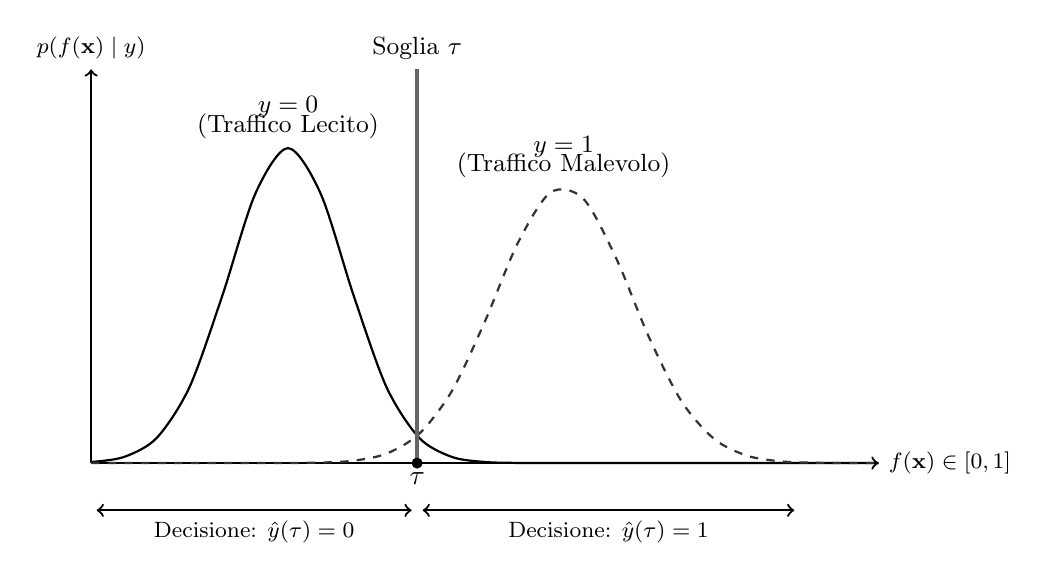
\begin{tikzpicture}[]
        % Assi cartesiani
        \draw[->, thick] (0,0) -- (10,0) node[right] {\footnotesize $f(\mathbf{x}) \in [0,1]$};
        \draw[->, thick] (0,0) -- (0,5) node[above] {\footnotesize $p(f(\mathbf{x}) \mid y)$};

        % Distribuzione Classe 0 (Lecito) - Linea continua
        \draw[thick, black, smooth, domain=0:10] plot (\x, {4.0*exp(-(\x-2.5)^2/1.1)});
        \node at (2.5, 4) [anchor=south, align=center] {
            \small $y=0$ \\[-5pt]
            \small (Traffico Lecito)
        };

        % Distribuzione Classe 1 (Malevolo) - Linea tratteggiata
        \draw[thick, dashed, black!80, smooth, domain=0:10] plot (\x, {3.5*exp(-(\x-6)^2/1.5)});
        \node at (6.0, 3.5) [anchor=south, align=center] {
            \small $y=1$ \\[-5pt]
            \small (Traffico Malevolo)
        };

        % Soglia decisionale tau
        \draw[very thick, gray!80!black] (4.14,0) -- (4.14,5);
        \node[above] at (4.14, 5) {\small Soglia $\tau$};
        \fill (4.14,0) circle (2pt) node[below] {$\tau$};

        % Regioni decisionali
        \draw[<->, thick, shorten >=2pt, shorten <=2pt] (0, -0.6) -- (4.14, -0.6) node[midway, below] {\footnotesize Decisione: $\hat{y}(\tau)=0$};
        \draw[<->, thick, shorten >=2pt, shorten <=2pt] (4.14, -0.6) -- (9, -0.6) node[midway, below] {\footnotesize Decisione: $\hat{y}(\tau)=1$};
    \end{tikzpicture}
    \caption{Mappatura della probabilità a posteriori $f(\mathbf{x})$ sulla regola decisionale binaria $\hat{y}(\tau)$ in funzione della soglia $\tau$.}
    \label{fig:soglia_decisionale}
\end{figure}

\subsubsection{Formalizzazione delle Metriche Derivate}
\label{subsubsec:metriche_derivate_formali}

Per rendere la valutazione indipendente dalla numerosità del campione di test, si introducono i principali tassi relativi derivati dalla matrice di confusione \cite{fawcett2006}:
\begin{equation}
    TPR(\tau)=\frac{TP(\tau)}{TP(\tau)+FN(\tau)},
    \qquad
    FPR(\tau)=\frac{FP(\tau)}{FP(\tau)+TN(\tau)}
\end{equation}

cui corrispondono i rispettivi complementari
\begin{equation}
\begin{aligned}
    FNR(\tau) &= 1-TPR(\tau) \\
              &= \frac{FN(\tau)}{TP(\tau)+FN(\tau)},
\end{aligned}
\qquad
\begin{aligned}
    TNR(\tau) &= 1-FPR(\tau) \\
              &= \frac{TN(\tau)}{TN(\tau)+FP(\tau)}.
\end{aligned}
\end{equation}

L'affidabilità delle segnalazioni generate dal classificatore è invece misurata dalla \textit{Precision}:
\begin{equation}
    Precision(\tau)=\frac{TP(\tau)}{TP(\tau)+FP(\tau)}
\end{equation}

Per sintetizzare il compromesso tra capacità di rilevamento degli attacchi e contenimento dei falsi allarmi si utilizza l'\textit{F1-score}, definito come media armonica tra Precision e Recall\footnote{Nei sistemi NIDS la media armonica è preferita alla media aritmetica poiché penalizza maggiormente modelli caratterizzati da un forte sbilanciamento tra sensibilità agli attacchi e precisione delle segnalazioni.}:
\begin{equation}
    F_1(\tau)=2\cdot\frac{Precision(\tau)\cdot TPR(\tau)}{Precision(\tau)+TPR(\tau)}
\end{equation}

Infine, l'\textit{Accuracy} rappresenta la proporzione complessiva di classificazioni corrette:
\begin{equation}
    Accuracy(\tau)=\frac{TP(\tau)+TN(\tau)}{N}
\end{equation}

Tale indicatore assume tuttavia un ruolo secondario nei problemi di intrusion detection, poiché non risulta sufficientemente informativo in presenza di distribuzioni fortemente sbilanciate tra traffico nominale e traffico malevolo.

\subsubsection{Dinamica della Soglia, Curve ROC/PR e Average Precision}
\label{subsubsec:analisi_grafica}

La valutazione puntuale delle metriche presuppone la scelta di uno specifico valore della soglia decisionale (ad esempio $\tau=0.5$). Una caratterizzazione più completa del comportamento discriminativo del classificatore richiede invece l'analisi dell'intero intervallo di valori della soglia, $\tau\in[0,1]$.

A tale scopo si impiegano la curva \textit{Receiver Operating Characteristic} (ROC) e la curva \textit{Precision--Recall} (PR). La prima viene sintetizzata mediante $AUC_{ROC}$, mentre per la seconda la pipeline utilizza l'\textit{Average Precision} (AP), calcolata come media pesata dei valori di Precision rispetto agli incrementi di Recall tra soglie successive:
\begin{equation}
    AUC_{ROC}=\int_{0}^{1}TPR\,d(FPR),
    \qquad
    AP=\sum_n (R_n-R_{n-1})P_n.
\end{equation}

\begin{figure}[H]
    \centering
    \begin{tikzpicture}[global_font]
        % --- Sottofigura (a): Curva ROC ---
        \begin{scope}[shift={(0,0)}]
            % Griglia di riferimento
            \draw[neutralgrey!30, thin] (0,4) -- (4,4) -- (4,0);
            \node[below left, text=neutralgrey] at (0,0) {\footnotesize $0$};
            \node[below, text=neutralgrey] at (4,0) {\footnotesize $1$};
            \node[left, text=neutralgrey] at (0,4) {\footnotesize $1$};

            % Area sottesa (AUC)
            \fill[lightblue] (0,0) -- plot[smooth, domain=0:4] (\x, {4*sqrt(\x/4)}) -- (4,0) -- cycle;

            % Baseline casuale (diagonale)
            \draw[dashed, accentorange, thick] (0,0) -- (4,4);

            % Curva ROC
            \draw[very thick, mainblue, smooth, domain=0:4] plot (\x, {4*sqrt(\x/4)});

            % Etichette
            \node[text=mainblue, font=\small\bfseries] at (2.3, 1.2) {$AUC_{ROC}$};
            \node[above, text=neutralgrey] at (2.5, 5) {\textbf{(a) Curva ROC}};

            % Assi
            \draw[arrow_flow] (0,0) -- (5,0) node[right, text=neutralgrey] {\footnotesize $FPR$};
            \draw[arrow_flow] (0,0) -- (0,5) node[above, text=neutralgrey] {\footnotesize $TPR$};
        \end{scope}

        % --- Sottofigura (b): Curva Precision-Recall ---
        \begin{scope}[shift={(7,0)}]
            % Griglia di riferimento
            \draw[neutralgrey!30, thin] (0,4) -- (4,4) -- (4,0);
            \node[below left, text=neutralgrey] at (0,0) {\footnotesize $0$};
            \node[below, text=neutralgrey] at (4,0) {\footnotesize $1$};
            \node[left, text=neutralgrey] at (0,4) {\footnotesize $1$};

            % Area sottesa (AUC)
            \fill[lightblue] (0,0) -- plot[smooth, domain=0:4] (\x, {4 - 2*(\x/4)^2}) -- (4,0) -- cycle;
            
            % Baseline prevalenza (linea orizzontale)
            \draw[dashed, accentorange, thick] (0,0.8) -- (4,0.8) node[right, text=accentorange] {\footnotesize $\pi$};

            % Curva PR
            \draw[very thick, mainblue, smooth, domain=0:4] plot (\x, {4 - 2*(\x/4)^2});

            % Etichette
            \node[text=mainblue, font=\small\bfseries] at (1.2, 1.2) {$AP$};
            \node[above, text=neutralgrey] at (2.5, 5) {\textbf{(b) Curva PR}};

            % Assi
            \draw[arrow_flow] (0,0) -- (5,0) node[right, text=neutralgrey] {\footnotesize $Recall\ (TPR)$};
            \draw[arrow_flow] (0,0) -- (0,5) node[above, text=neutralgrey] {\footnotesize $Precision$};
        \end{scope}
    \end{tikzpicture}
    \caption{Rappresentazione schematica delle curve ROC (a) e Precision--Recall (b). L'area è illustrativa; la sintesi numerica della curva PR impiegata nella pipeline è l'Average Precision (AP).}
    \label{fig:curve_roc_pr}
\end{figure}

L'indice $AUC_{ROC}$ sintetizza la capacità discriminativa lungo la curva ROC, mentre l'Average Precision (AP) riassume la relazione Precision--Recall e risulta informativa in presenza di classi asimmetriche \cite{saito2015}.

\subsubsection{Degrado Prestazionale e Significatività Statistica (Welch's t-test)}
\label{subsubsec:significativita_statistica}

Il trasferimento di un modello tra domini caratterizzati da differenti distribuzioni marginali delle caratteristiche $P(\mathbf{x})$ (\textit{covariate shift}) può determinare una degradazione delle prestazioni di classificazione \cite{pan2010}. Tale variazione dell'efficacia discriminativa di un modello $M$, valutato sul dominio sorgente $\mathcal{D}_S$ e sul dominio target $\mathcal{D}_T$, può essere espressa come
\begin{equation}
    \Delta F_1=F_1(M,\mathcal{D}_S)-F_1(M,\mathcal{D}_T).
\end{equation}

Per la verifica inferenziale delle differenze tra configurazioni si utilizza il protocollo di Welch già formalizzato nella Sottosezione~\ref{subsubsec:welch_test}. La procedura viene interpretata in chiave esplorativa e secondo le assunzioni del test implementato, senza attribuire al rigetto dell'ipotesi nulla un significato causale.

\section[Sintesi del Capitolo e Raccordo con la Campagna Sperimentale]{Sintesi del Capitolo e Raccordo con la Campagna \\\ Sperimentale}
\label{sec:sintesi_raccordo_ch4}

L'impalcatura teorica e metodologica formalizzata nel presente capitolo definisce un modello astratto e rigoroso per la valutazione dei sistemi NIDS soggetti a \textit{domain shift}. 
Attraverso l'allineamento degli spazi delle \textit{feature}, la formalizzazione delle configurazioni di classificazione aggregate e specialistiche e la definizione di un protocollo \textit{multi-seed}, il framework consente di caratterizzare separatamente la variabilità inter-seed e il confronto inferenziale esplorativo tra configurazioni.

Tuttavia, la validità dei vincoli analitici e delle proprietà di invarianza descritte richiede un riscontro quantitativo su scenari operativi concreti. 
Nel Capitolo~\ref{ch:implementazione}, il framework teorico viene tradotto nell'architettura software e nel protocollo operativo adottati per la campagna sperimentale. I risultati prodotti da tale implementazione sono invece analizzati separatamente nel Capitolo~\ref{ch:risultati}.